% An MSI thesis template thrown together Oct 2005 - CW

% openany allows a chapter to start on even numbered pages
\documentclass[a4paper,12pt,openany]{book}


  % a file containing your definitions, which packages to load etc
  \usepackage{definitions}
  % line-spacing factor
  \renewcommand{\baselinestretch}{1.2}

  % use this if you don't want headers and page numbers on
  % blank pages at the end of chapters
  \newcommand{\blanknonumber}{\newpage\thispagestyle{empty}}

  % margins
  \setlength{\voffset}{-1in}
  \setlength{\hoffset}{-1in}
  \setlength{\oddsidemargin}{4cm}
  \setlength{\evensidemargin}{2.5cm}
  \setlength{\textwidth}{14.5cm}
  \setlength{\textheight}{22.5cm}
  \setlength{\topmargin}{2.5cm}


  % for working drafts, un-comment the following command and list
  % the chapters etc you want to see in the output, eg
  % \includeonly{titlepage,chapter1,chapter2}



\begin{document}


% set page numbers to roman and suppress chapter numbers
\frontmatter


% remove or switch the order of these as you see fit
\begin{titlepage}
\begin{center}

\vspace*{\fill} \Huge
                        Thesis title
\\
\vfill\vfill\Large
                          Your name
\\
\vfill\vfill
                          Month Year
\\
\vfill\vfill \normalsize
         A thesis submitted for the degree of Doctor of Philosophy\\
         of the Australian National University
\vfill
         
\includegraphics{ANU.eps}

\end{center}

\end{titlepage}
%\blanknonumber


\blanknonumber\ \blanknonumber

\vspace*{\fill}

\begin{center}\emph{
%
For someone or something or whatever
%
}
\end{center}

\vfill\vfill\vfill
%\blanknonumber

\chapter*{Declaration}\label{declaration}
\thispagestyle{empty}
The work in this thesis is my own except where otherwise stated.

\vspace{1in}


\hfill\hfill\hfill
%
Your name
%
\hspace*{\fill}
%\blanknonumber

\chapter*{Acknowledgements}\label{acknowledgements}
\addcontentsline{toc}{chapter}{Acknowledgements}


% your acknowledgements go here
%\blanknonumber
\chapter*{Abstract}\label{abstract}

\addcontentsline{toc}{chapter}{Abstract}

Donaldson-Witten theory is Witten's supersymmetric topological quantum field
theory that realises the Donaldson invariants of smooth 4-manifolds as
correlation functions of certain operators. This thesis culminates with a
detailed exposition of the differential geometric interpretation of this 
formulation by Atiyah and Jeffrey.
They show that the action of the theory can be understood as an
infinite dimensional analogue of the Chern-Gauss-Bonnet formula for the Euler
characteristic of a vector bundle. The bulk of this thesis introduces the background
necessary to understand this. The framework of equivariant cohomology is
used to derive the Mathai-Quillen representative of a universal 
Thom form. We then demonstrate its application to localisation
of integrals, starting with a proof of the Poincar\'e-Hopf theorem and
proceeding to arbitrary vector bundles. Finally, the construction of Donaldson 
invariants is sketched before expounding the Atiyah-Jeffrey interpretation. 



%\blanknonumber
\tableofcontents%\blanknonumber


\chapter{Notation and terminology}\label{notation}
%\addcontentsline{toc}{chapter}{Notation and terminology}

\renewcommand{\thefootnote}{\fnsymbol{footnote}}



Some preliminary description here?  Eg, ``In the following, $G$ is
a group, $H$ is a subgroup of $G$, \ldots''
\vspace{2em}


\noindent\textbf{Notation}

% adjust the lengths to suit your needs (difference of .22cm works best)

\newcommand{\nttn}[2]{\item[{\ \makebox[3.18cm][l]{#1}}]{#2}}
\begin{list}{}{ \setlength{\leftmargin}{3.4cm}
                \setlength{\labelwidth}{3.4cm}}

\nttn{notation}{definition text goes here definition text goes
                here definition text goes here}

\nttn{notation}{definition text goes here definition text goes
                here definition text goes here}

\nttn{notation}{definition text goes here definition text goes
                here definition text goes here}

\end{list}

\

\noindent\textbf{Terminology}

% adjust the lengths to suit your needs (difference of .22cm works best)

\newcommand{\term}[2]{\item[{\ \makebox[4.58cm][l]{#1}}]{#2}}
\begin{list}{}{ \setlength{\leftmargin}{4.8cm}
                \setlength{\labelwidth}{4.8cm}}

\term{terminology}{definition text goes here definition text goes
                   here definition text goes here}

\term{terminology}{definition text goes here definition text goes
                   here definition text goes here}

\term{terminology}{definition text goes here definition text goes
                   here definition text goes here}

\end{list}
%\blanknonumber



% set page numbers to arabic, reset to 1
\mainmatter
\renewcommand{\thefootnote}{\arabic{footnote}}

% assuming there are files chapter1.tex etc...

\chapter{Chapter title goes here}
\label{chapter1}



Blah blah blah...

The environments below all use the same numbering sequence.  See
the file \verb+definitions.tex+ if you want to change this.

\begin{defn}
A lemma.
\end{defn}

\begin{notn}
Some notation.
\end{notn}

\begin{lemma}
A lemma.
\end{lemma}

\begin{theorem}
A theorem.
\end{theorem}

\begin{proof}
A proof.
\end{proof}

\begin{cor}
A corollary.
\end{cor}

\begin{prop}
A proposition.
\end{prop}

\begin{ex}
An example.
\end{ex}

\begin{question}
A question.
\end{question}

\begin{remark}
A remark.
\end{remark}


\newpage

Blah blah blah...

%\chapter{Equivariant Cohomology}
\label{chapter2}

\section{Preliminaries}
Equivariant differential topology extends the results of differential topology
to manifolds/topological spaces with a group action, called a $G$-space. A
$G$-space is a topological space $X$ with a continuous action $X\times G \to X$ 
such that $x\cdot e = x$ for $e$ the identity in  $G$ and $(x\cdot g) \cdot h =
x\cdot (gh)$ for $g,h\in G$. 

We will often be dealing with both left and right group actions, but these are
equivalent. If we have a right $G$ action on $X$, this can be turned into a left
action by defining  $g \cdot x = x \cdot g^{-1}$, so that $h\cdot (g\cdot x) =
(x\cdot g^{-1})\cdot h^{-1} = x\cdot (g^{-1}h^{-1}) = (hg)\cdot x$. The same
argument works in the other direction.


There are two definitions of equivariant
cohomology: the Borel construction which uses classifying spaces, and the Cartan model.
These have been proven to be equivalent in the case of compact manifolds with
compact group actions by Cartan. % TODO reference theorem, venselaar

First let us recall some basic definitions in algebraic topology.
\begin{defn}
	Let $(X,x_0)$ and $(Y,y_0)$ are based topological spaces. Two maps
	$f,g:(X,x_0)\to(Y,y_0)$ are \underline{homotopic} if there is a continuous
	map $F:X\times [0,1]\to Y$ such that
	$F(x,0)=f(x),F(x,1)=g(x),F(x_0,t)=y_0$. Then we denote $f\sim g$.

	A \underline{homotopy equivalence} is a continuous map $f:(X,x_0)\to(Y,y_0)$
	that has a homotopy inverse, i.e. a continuous map $g:(Y,y_0)\to(X,x_0)$
	such that $f\circ g \sim \mathbb{1}_Y$ and $g\circ f \sim \mathbb{1}_X$.
	Then we say $X$ and  $Y$ have the same homotopy type.

	A topological space $(X,x_0)$ is \underline{contractible} if it has the
	homotopy type of a point. 
	A space $X$ is \underline{weakly contractible} if all its homotopy groups
	are trivial, i.e.  $\pi_q(X)=0$ for all  $q\geq 0$. 
\end{defn}
An important theorem in homotopy theory is Whitehead's theorem, which states
that if a continuous map $f:X\to Y$ of CW complexes induces an isomorphism on
all homotopy groups, then  $f$ is a homotopy equivalence. In particular, this
means that a weakly contractible CW complex is contractible, using the inclusion
map $x_0 \to X$.
% every smooth manifold is homotopy equivalent to a CW complex pg 18 Tu

A useful tool for computing homotopy groups is the homotopy exact sequence of a
fiber bundle. 
\begin{thm}[{\cite[Thm 4.41]{hatcher}}] \label{thm:fiber_les}
	Suppose $(E,x_0) \xrightarrow{\pi} (B,b_0)$ is a fiber bundle with fiber
	$F=\pi^{-1}(b_0)$ and path-connected base space $B$. Let  $x_0$ also be the
	basepoint of $F$, and  $i:(F,x_0)\to (E,x_0)$ the inclusion map. Then there
	exists a long exact sequence
	\[
		\ldots\to\pi_n(F,x_0) \xrightarrow{i_*}\pi_n(E,x_0)
		\xrightarrow{\pi_*}\pi_n(B,b_0)
		\to \pi_{n-1}(F,x_0)\to\ldots\to\pi_0(E,x_0)\to 0
	\] 
	All maps are group homomorphisms except the last three maps which are set
	maps.
\end{thm}

In this section, assume $G$ is a topological group. 
Cartan's mixing contruction, also
called Borel's construction, turns a principal  $G$-bundle and a  $G$-space  $M$
into a fiber bundle with fiber  $M$. 

If  $P$ is a right  $G$-space and  $M$ is a left  $G$-space, the 
\underline{Cartan mixing space} of  $P$ and  $M$ is the quotient 
$P\times_G M:= (P\times M) / \sim$ by the 
equivalence relation $(p,m)\sim (pg,g^{-1}m) \textrm{ for some }g\in G$.
Equivalently, this is the orbit space $(P\times M) /G$ under the diagonal action
$g(p,m) = (pg,g^{-1}m)$.

If in addition $P\xrightarrow{\pi} B$ is a principal $G$-bundle, define the projection
$\tau_1:P\times_GM\to B$ by $\tau_1([p,m])=\pi(p)$. This is well defined because
$\pi$ preserves the fiber.

\begin{prop} \label{prop:cartan_mixing}% prop 4.5 Tu
	If $P\xrightarrow{\pi} B$ is a principal  $G$-bundle and  $M$ is a left  $G$-space,
	then  $\tau_1 : P\times_G M\to B$ is a fiber bundle with fiber  $M$.
\end{prop}
\begin{proof}
	Suppose $\pi^{-1}(U)\simeq U\times G$. It suffices to show
	$\tau_1^{-1}(U)\simeq U\times M$. 
	\begin{align*}
		\tau_1^{-1}(U)
		&= \{[p,m]\in P\times_GM \mid \pi(p)\in U\} \\
		&= \pi^{-1}(U)\times _G M \\
		&\simeq (U\times G) \times_G M 
	\end{align*}
	To show this is homeomorphic to $U\times M$, we define 
	$\varphi:(U\times G) \times_G M \to U\times M$ by 
	$[(x,g),m] \mapsto (x,gm)$. It has inverse $(x,m)\mapsto [(x,1),m]$.
\end{proof}


\section{Borel construction}
\begin{defn}
	Given a topological group $G$, let  $EG \to BG$ be a principal  $G$-bundle
	with weakly contractible total space  $EG$. Define the  \underline{homotopy
	quotient} of a $G$-space $M$ by $M_G:=EG\times_G M$.
	 
	The \underline{equivariant cohomology} of $M$ is defined to be the singular
	cohomology of the homotopy quotient: $H_G^*(M;R) := H^*(M_G;R)$.
\end{defn}
Of course, for this definition to make sense we need to show that it is
independent of the choice of weakly contractible $EG$, which we do now. 

\begin{defn}
	A map $f:X\to Y$ is a \underline{weak homotopy equivalence}
	it induces an isomorphism of homotopy groups
	$f_*:\pi_q(X)\to\pi_q(Y)$ for all  $q\geq 0$. 
\end{defn}

\begin{lem} % lemma 4.9 Tu
	If $E$ is a weakly contractible $G$-space, and $P\to P/G$ is a principal
	$G$-bundle, there is a weak homotopy equivalence $(E\times P) /G \to P /G$.  
\end{lem}
\begin{proof}
	We consider $E\times_G P = (E\times P) /G$ as the orbit space under 
	the diagonal action $(e,p)g = (g^{-1}e,pg)$. 
	By Proposition \ref{prop:cartan_mixing}, $(E\times P) /G \to P /G$ is a
	fiber bundle with fiber $E$. By the long exact sequence of a fiber
	bundle (Theorem \ref{thm:fiber_les}), the sequence of induced maps
	\[
	\ldots \to \pi_q(E) \to \pi_q((E\times P) /G) \to\pi_q(P /G) \to
	\pi_{q-1}(E)\to \ldots
	\] 
	is exact. Since $E$ is weakly contractible, the middle map is an isomorphism
	 $\pi_q((E\times P) /G) \to \pi_q(P /G)$ for any  $q\geq 0$.
\end{proof}

\begin{cor}
	Suppose $M$ is a left  $G$-space. If $E\to B$ and  $E'\to B'$ are two principal
	$G$-bundles with weakly contractible total spaces, then $E\times_G M$ and
	$E'\times_G M$ are weakly homotopy equivalent.
\end{cor}
\begin{proof}
	Note that homotopy equivalence is not a symmetric relation, but by symmetry
	of $E$ and  $E'$ both directions hold. 
	Applying the previous lemma to $E$ and $E'\times M$, there is a weak
	homotopy equivalence $(E\times E'\times M)/G$ to $(E'\times M) /G$.

\end{proof}
\begin{thm}[{\cite[Proposition 4.21]{hatcher}}]
	A weak homotopy equivalence $f:X\to Y$ induces isomorphisms
	$f^*:H^n(Y;R)\to H^n(X;R)$ in cohomology for all  $n$.
\end{thm}

Hence, combining the last two results tells us that for any two choices of
weakly contractible principal $G$-bundles  $E$ and  $E'$,  $H^*(E\times_G M)
\simeq H^*(E'\times_G M)$ so the definition of equivariant cohomology is
independent of the choice of  $E$. 

To define the equivariant cohomology of a $G$-space  $M$, we need a weakly
contractible principal $G$- bundle $EG$. It turns out that for CW complexes,  
a weakly contractible $G$-bundle is equivalent to a universal $G$-bundle, as
defined below.
\begin{defn}
	A principal $G$-bundle  $\pi:EG\to BG$ is a \underline{universal $G$-bundle} 
	if the following two conditions hold:
	\begin{enumerate}[(i)]
	    \item for any principal $G$-bundle  $P$ over a CW complex $X$, there
			exists a continuous map  $h:X\to BG$ such that  $P \simeq h^*EG$ 
		\item If $h_0,h_1:X\to BG$ and $h_0^*EG \simeq h_1^*EG$ over a CW
			complex $X$, then  $h_0$ and $h_1$ are homotopic
	\end{enumerate}
	The base space $BG$ of a universal  $G$-bundle is called a
	\underline{classifying space} for  $G$.
\end{defn}
\begin{thm}[Steenrod 1951] % thm 5.2 Tu
	Let $E\to B$ be a principal  $G$-bundle. If  $E$ is weakly contractible,
	then  $E\to B$ is a universal bundle. Conversely, if  $E\to B$ is a
	universal bundle and  $B$ is a CW complex, then  $E$ is weakly contractible.
\end{thm}

\begin{comment}
Let $X$ be a CW complex, and $[X,B]$ be the homotopy classes of maps $h:X\to B$, 
and  $\mathcal{P}_G(X)$ be the isomorphism classes of principal $G$-bundles over $X$. 
Then the definition of universal $G$-bundle states the map
$\varphi:[X,BG]\to\mathcal{P}_G(X)$ given by $h\mapsto h^*(EG)$ is surjective
(condition (i)) and injective (condition (ii)). 
% TODO: well defined by Theorem 5.3 Tu
\end{comment}

\begin{thm} %thm 5.6
	If a CW classifying space exists for a topological group $G$, it is unique 
	up to homotopy equivalence.
\end{thm}
\begin{proof}
	Suppose $E\to B$ and  $E'\to B'$ are universal bundles, where $B$ and  $B'$
	are CW complexes. Since  $E'$ is
	universal there is a map  $f:B\to B'$ such that  $E'\simeq h^*E$. Similarly
	there is a map  $h:B'\to B$ such that  $E\simeq h^*E'$. Therefore,  $E\simeq
	f^*h^*E=(h\circ f)^*E$. 

	But this means  $(h\circ f)^*E = \id_B^*E$, so by condition (ii) of a
	universal bundle, $h\circ f \simeq \id_B$. Similarly, $f\circ h\simeq
	\id_{B'}$. Therefore $B$ and  $B'$ are homotopy equivalent.
\end{proof}

Moreover, it can be shown that a universal $G$-bundle exists for any topological
group  $G$. % Milnor's construction TODO: elaborate?


\section{Cartan model}
\begin{defn} \label{def:contraction} % BGV
	If $V$ is a vector space, the \underline{contraction} (or interior
	multiplication) operator $\iota(v) :
	\Lambda V^* \to \Lambda V^*$ for $v\in V$ is the unique operator such that
	\begin{enumerate}[(1)]
	    \item $\iota(v)\alpha = \alpha(v)$ if  $\alpha\in V^*$
		\item $\iota(v)(\alpha\wedge\beta) = (\iota(v)\alpha)\wedge\beta + 
			(-1)^{\abs{\alpha}}\alpha\wedge(\iota(v)\beta)$, if  $\alpha,\beta$
			are homogeneous elements of  $\Lambda V^*$.
	\end{enumerate} % mention exterior operator?
\end{defn}
Hence, we can define \underline{interior multiplication} with a vector
field as the map $\iota(X) : \Omega^*(M) \to \Omega^{*-1}(M)$.
The definition similarly extends to vector valued forms.
\begin{thm} % thm 10.4 tu equivariant, p18 BGV
	Let $X$ be a vector field on  $M$, and $\alpha\in \Omega(M)$. 
	\begin{enumerate}[(i)]
	    \item $\mathcal{L}(X)d = d\mathcal{L}(X)$
		\item $\mathcal{L}(X)(\iota(Y)\alpha) = \iota([X,Y])\alpha +
			\iota(Y)(\mathcal{L}(X)\alpha)$ 
		\item Cartan's homotopy formula: $\mathcal{L}(X) = d
			\cdot\iota(X)+\iota(X)\cdot d$
	\end{enumerate}
\end{thm}
\begin{proof}
	
\end{proof}

\begin{defn}
	Let $\mathfrak{g}$ be a Lie algebra. A \underline{$\mathfrak{g}$-differential graded
	algebra} is a commutative graded algebra $\Omega= \bigoplus_{k\geq
	0}\Omega^k$ with 
	\begin{itemize}
		\item an antiderivation $d:\Omega\to\Omega$ of degree 1 such that
	$d\circ d = 0$
		\item two actions of $\mathfrak{g}$: $\iota:\mathfrak{g}\times\Omega\to\Omega$
			and  $\mathcal{L}:\mathfrak{g}\times\Omega\to\Omega$, where for
			$X\in\mathfrak{g}$,  $\iota_X$ and  $\mathcal{L}_X$ are
			$\mathbb{R}$-linear in $X$,  $\iota_X$ acts on  $\Omega$ as an
			antiderivation of degree -1,  $\iota_x = 0$, and  $\mathcal{L}_X$
			acts as a derivation of degree 0.
	\end{itemize}
	Furthermore, the operators satisfy Cartan's homotopy formula:
	$\mathcal{L}_X= d\iota_X+\iota_Xd$.
\end{defn}
Note that commutativity for a graded algebra means that if $a\in
\Omega^k,b\in\Omega^l$ then $ba = (-1)^{kl}ab$.  

\begin{defn}
	A differential form $\alpha\in\Omega$ is 
	\underline{horizontal} if $\iota_X\alpha=0$ for all $X\in\mathfrak{g}$. 
	It is \underline{invariant} if $\mathcal{L}_X\alpha = 0$ for all $X\in
	\mathfrak{g}$. It is \underline{basic} if it is both horizontal and
	invariant.
\end{defn}
Note that in the case of a principal bundle, we think of $X\in \mathfrak{g}$ as 
a vertical vector field via $X_p = \odv{}{t}_{t=0} p \exp (t X)$. 
\begin{comment} %%% stuff about principal and associated bundles
\begin{defn}
	A differential form $\alpha\in\Omega(P,V)$ on a principal $G$-bundle  with 
	representation $(V,\rho)$ is \underline{$\rho$-equivariant}   
	if for every $g\in G$, $r_g^*\alpha = \rho(g^{-1})\alpha$. 
	\\
	A differential form $\alpha\in\Omega(P,V)$ on a principal $G$-bundle  with 
	representation $(V,\rho)$ is \underline{basic}  
	if it is horizontal and $\rho$-equivariant. This subspace is
	denoted $\Omega_{bas}(P,V)$.
\end{defn}
Let $P$ be a principle $G$-bundle, and let ($V,\rho$) be a representation of
$G$. Let $E= P\times_\rho V$ be the associated bundle.
\begin{thm} %thm 31.9 tu
	The map $\Omega_{bas}^k(P,V) \to \Omega^k(M,P\times_\rho V)$ given by 
	$\omega \mapsto \alpha_x = f_p \circ \omega_p$
	is a linear isomorphism, where $f_p: V\to E_x$ is the isomorphism  $v\mapsto
	[p,v]$, and $p\in\pi^{-1}(x)$ is any point.
\end{thm}

\begin{cor} % Prop 1.7 BGV
	There is a natural isomorphism between $\Gamma(M,P\times_\rho V)$ and
	$\rho$-equivariant maps in
	$C^{\infty}(P,V)$, given by sending $s\in C^{\infty}(P,V)^G$ to $s_M$
	defined by  $s_M(x) = [p,s(p)]$, where  $p\in\pi^{-1}(x)$ is any element.
\end{cor}


Recall that a \underline{vertical vector} on a fibre bundle $E$ with base  $M$
is a tangent vector  $X\in TE$ such that  $X(\pi^* f) = 0$ for any  $f\in
C^\infty(M)$. The space $V_pP$ of vertical tangent vectors to a point $p$ in a
principal $G$-bundle can be canonically identified with the Lie algebra $\mathfrak{g}$ 
of $G$ in the following way. 
If $X\in\mathfrak{g}$, the \underline{fundamental vector field} associated to
$X$, denoted $X_P \in \Gamma(VP)$, is
 \[
X_P = \odv{}{t}_{t=0} p \exp (t X)
\] 
This is a vertical vector field because $X_P(\pi^*f) = \odv{}{t}_{t=0} f(p \exp
(t X)) = 0$. 
\end{comment}


\begin{prop} % prop 18.10 tu
	If $\Omega$ is a  $\mathfrak{g}$-differential graded algebra, the vector
	space of basic elements $\Omega_{bas}$ is a $\mathfrak{g}$-differential
	graded algebra.
\end{prop}
% TODO tensor product of dgas
Tensor prouct of dgas is a dga

\begin{thm}[Equivariant de Rham theorem] % 19.4 Tu
	For a compact connected Lie group $G$ with Lie algebra $\mathfrak{g}$, and
	$G$-manifold  $M$, there is a graded-algebra isomorphism 
	 \[
		 H_G^*(M) \simeq H^*((W(\mathfrak{g})\otimes \Omega(M))_{bas}, \delta)
	\] 
\end{thm}
The complex $(W(\mathfrak{g})\otimes \Omega(M))_{bas}$ with the Weil
differential is called the \underline{Weil model}.

\begin{thm}[Weil-Cartan isomorphism] % Thm 21.1 Tu
	Let $G$ be a connected Lie group, and $M$ be a left $G$-manifold. There is a
	graded-algebra isomorphism 
	\[
		F : (W(\mathfrak{g})\otimes \Omega(M))_{hor} \to S(g^*\otimes \Omega(M))
	\] 
	\[
	a+ \sum \theta_I a_I \mapsto a
	\] 
	which induces a graded-algebra isomorphism on the basic algebras
	$F : F : (W(\mathfrak{g})\otimes \Omega(M))_{bas} \to (S(g^*\otimes
	\Omega(M)))^G$. 
\end{thm}
The complex $(S(g^*\otimes \Omega(M)))^G$ is called the \underline{Cartan
model}. Elements of the Cartan model are called \underline{equivariant forms}.

\section{BRST Model}
In the context of topological field theories, another model of equivariant
cohomlogy arises naturally, called the BRST model. As a vector space, it is
identical to the Weil model $W(\mathfrak{g})\otimes \Omega(M)$, but with
differential $d_B = d_W + \theta^i\otimes \mathcal{L}_i - u^i \otimes \iota_i$.

% TODO how does it arise? proof of conjugagion theorem, why conjugate?
It was shown by Kalkman that the BRST and Weil models are related by the algebra
automorphism of conjugation by $\exp (\theta^i \iota_i)$. 


\section{Equivariant characteristic classes}
\begin{defn} % from ch1 BGV
	Let $\pi: E\to M$ be a fibre bundle and let $G$ be a Lie group. We say $E$
	is a \underline{$G$-equivariant bundle} if $E$ and  $M$ are 
	$G$-manifolds  with $g \cdot \pi = \pi \cdot g$ for all  $g\in G$.\\
	If  $E$ is a vector bundle, we further require that the action  $g: E_x \to
	E_{gx}$ is linear.
\end{defn}

\begin{prop} % prop 9.4 Tu
	Let $f:M\to N$ be a $G$-equivariant map of  $G$-spaces, and let
	$f_G:M_G\to N_G$ be defined by $[e,x]\mapsto [e,f(x)]$. 
	\begin{enumerate}[(i)]
	    \item If $f$ is injective, then $f_G$ is injective
		\item If $f$ is surjective, then $f_G$ is surjective
		\item If $M\xrightarrow{f} N$ is a fiber bundle with fiber $F$, then
			$M_G\xrightarrow{f_G}N_G$ is a fiber bundle with fiber  $F$. 	
	\end{enumerate}
\end{prop}

Let $G$ be a topological group, and  $\pi : E\to M$ be a  $G$-equivariant vector
bundle. By the proposition above, this induces a vector bundle  $\pi_G : E_G\to
M_G$ on homotopy quotients of the same rank. If $E\to M$ is oriented, then so is
$E_G \to M_G$. 

The \underline{equivariant Euler class} of an oriented equivariant vector bundle
$\pi : E \to M$ is defined to be the Euler class of $\pi_G : E_G \to M_G$, i.e.
it is an element of $H_G^*(M)$. 



%
\chapter{Mathai-Quillen formula}
\label{chapter3}
The Mathai-Quillen formula is an explicit differential form representative of 
the Thom class of a vector bundle. The significance of the Thom class is 
that its pullback to the base manifold gives a representative of the Euler
class, thus it can be used to calculate the Euler number.  
Recall that there are two quite different approaches for calculating the Euler number
$\chi(X) = \chi(TX)$ of an oriented even dimensional manifold $X$. 
This first is topological, and counts
the signed isolated zeros of a vector field on $X$, via the Poincar\'e-Hopf theorem. The
second is differential geometric and represents  $\chi(X)$ as the integral over
$X$ of a density constructed from the curvature of a connection on $X$, via
the Gauss-Bonnet theorem. 
The Mathai-Quillen representative of the class depends on both a section $s$ and 
connection  $\nabla$ on the vector bundle, and can be regarded as a formula 
which interpolates between the two approaches.  

Our interest in the formula is further motivated by its application in providing a
geometric interpretation of the action principle of Witten's TQFT, where he
characterised Donaldson invariants as correlation functions of observables, as
we will see later in Chapter \ref{chapter4}. 

\section{Integration along the fiber} \label{section:fiber_integration}
Let $\pi: E\to B$ be an oriented fiber bundle over a manifold $B$ with oriented
fiber $F$. Suppose $\dim F = m$ and $\dim B = n$.
\begin{defn}
	\underline{Integration along the fiber} is a map $\pi_* : \Omega^*(E)\to
	\Omega^{*-m}(B)$, defined as follows. Let $\alpha\in \Omega^k(E)$ and
	$v_1,\ldots,v_{k-m} \in T_bB$ 
	\[
	(\pi_*\alpha)_b(v_1,\ldots,v_{k-m}) = \int_{\pi^{-1}(b)}
	\alpha(\widetilde{v}_1,\ldots,\widetilde{v}_{k-m},-)
	\] 
	where $\widetilde{v}_i$ is any lift of $v_i$ to $TE$. 
The integral is computed by pulling back the form via a trivialisation $\phi 
:F \xrightarrow{\simeq} \pi^{-1}(b)$. 
\end{defn}
\begin{figure}[htb]
	\hfill
	\begin{minipage}[c]{0.5\textwidth}
	
\includegraphics[trim={5cm 5mm 5cm 3mm},clip,width=\textwidth]{figs/fiber_integral.pdf}
	\end{minipage} 
	\begin{minipage}[c]{0.44\textwidth}
	\caption{Lift of tangent vectors along $\pi^{-1}(b)$}
	\label{fig:fiber_integral}
	\end{minipage} 
\end{figure}
To show that this is well defined, we need to check 
\begin{itemize}
	\item the integral is independent of choice of trivialisation
	\item definition is independent of the choices of lifts
	\item integrand is a smooth differential form on $\pi^{-1}(b)$
	\item $\pi_*\alpha$ is a smooth differential form on $B$
\end{itemize}
Denote $\beta = \alpha(\widetilde{v}_1,\ldots,\widetilde{v}_{k-m},-)$.\\
(1) Choice of trivialisation. This comes from the fact that the trivialisation
is oriented: if $\phi_1,\phi_2 : F \to \pi^{-1}(b)$ are two trivialisations,
then $\psi:=\phi_1^{-1}\phi_2 : F \to F$ is an orientation preserving diffeomorphism. 
Hence, on an open subset $V_\alpha \subset F$ the integral is written in
coordinates as  
\[
\int_{V_{\alpha}} \phi_1^*\beta \odif{f_1}\ldots\odif{f_m} 
= \int_{V_\alpha} \psi^*\phi_1^*\beta  \odif{g_1}\ldots\odif{g_m}
\] 
where $g_i = \psi(f_i)$ are the transformed coordinate functions. Since
$\det(D\psi)=1$ by assumption, the two integrals are equal by the change of 
coordinates theorem. 

Moreover, for vector bundles and principal bundles, the definition is also 
independent of the choice of oriented trivialisation with the same orientation. 
Even if $\phi_1,\phi_2$ are taken from different trivialisations, the
transition function $\phi_1^{-1}\phi_2: F \to F$ will be an orientation
preserving diffeomorphism due to the extra structure on $\phi_1$ and
$\phi_2$, i.e. linear isomorphism or $G$-equivariant map. 

(2) Choice of lifts. Fix $a\in \pi^{-1}(b)$, and let $\widetilde{v}_1'$ be 
another lift of $v_1\in T_bB$. That is, 
$D\pi|_a(\widetilde{v}_1)=D\pi|_a(\widetilde{v}_1')=v_1$. So
$\widetilde{v}_1'-\widetilde{v}_1\in \ker D\pi|_a = T_a(p^{-1}(b))$.  

Since the fiber dimension is $m$, $m+1$ vectors 
$w_1,\ldots,w_m,\widetilde{v}_1'-\widetilde{v}_1 \in T_a(\pi^{-1}(b))$ are
linearly dependent, and therefore 
\[
\alpha(\widetilde{v}_1'-\widetilde{v}_1,
\widetilde{v}_2,\ldots,\widetilde{v}_{k-m},w_1,\ldots,w_m) = 0
\] 
which shows the integrand is independent of the choice of lifts.

(3) Integrand is smooth on $\pi^{-1}(b)$. Since $\alpha$ is a smooth 
differential form, we only need to check that its dependence on the lifted 
vectors is smooth. Given a local trivialisation $\phi : U\times F
\xrightarrow{\simeq} \pi^{-1}(U)$, at $a\in\pi^{-1}(b)$ we can choose the lift 
$\widetilde{v}_1 = D\phi|_{\phi^{-1}(a)}(v_1)$. This is a smooth choice, and
hence $\alpha$ is smooth by part (2). 

(4) $\pi_*\alpha$ is a smooth differential form on $B$. To see this, we can
write it out in coordinates. Let 
$dx_1,\ldots,dx_{n},dt_1,\ldots,dt_m \in T^*E|_U$ be a basis, where
$t_i$ are coordinate functions for $F$ and $x_i$ are coordinate functions for
$B$. Assume $\alpha$ is a product of 1-forms and has a factor of 
$dt_1\wedge \cdots\wedge dt_m$, since
otherwise $\beta$ will not be a top form on $\pi^{-1}(b)$. Then integration
along the fiber is locally described by 
\[
\alpha = \pi^*\eta \wedge f(x,t) \odif{t_1}\cdots \odif{t_m}   
\mapsto \eta\wedge \int_{\pi^{-1}(b)} f(x,t) \odif{t_1}\cdots \odif{t_m}
\] 
for some $\eta\in \Omega(B)$. It is now apparent that the dependence on $x$,
i.e. the coordinates for  $B$, is smooth. 
\begin{remark}
	Note that not all differential forms in $\Omega^*(E)$ are integrable, 
	so we typically restrict $\pi_*$ to forms which
	are compactly supported, compactly supported along the fiber, or rapidly
	decreasing. 
\end{remark}
In this chapter, we are interested in integration along the fiber for oriented
vector bundles in particular, however the general definition will be needed
later when we integrate over $G$-orbits of principal bundles. The case of vector
bundles is slightly simpler, because the fiber has global coordinates. 
\begin{prop} % Bott Tu p62
	Integration along the fiber $\pi_*$ commutes with the exterior derivative
	$d$.
\end{prop}
\begin{proof}
	Since $\pi_*$ and  $d$ are linear,
	it suffices to prove this proposition on the restriction $E|_U \simeq
	U\times F$ to a subset in the trivialising open cover. If $\omega\in
	\Omega_{cv}^*(E)$, to write it in coordinates we need to further choose a
	subset $U\times V$ which is diffeomorphic to an open neighbourhood of
	$\mathbb{R}^{n+m}$. Then
	we can write it locally as $\omega = \pi^*\eta \wedge f(x,t) dt_1\cdots
	dt_n$ for some $\eta\in \Omega^*(B)$. Then 
	\begin{align*}
		d\pi_*\omega
		&= d \paren{\eta\wedge \int f(x,t)\odif{t_1}\cdots\odif{t_m} } \\
		&= d\eta\wedge\int f(x,t)\odif{t_1}\cdots\odif{t_m}  
		+\eta\wedge \sum_i dx_i\int \partial_{x_i} f(x,t)\odif{t_1}\cdots\odif{t_m} 
	\end{align*}
	and 
	\begin{align*}
		\pi_*d\omega
		&= \pi_*\paren[2]{\pi^*d\eta\wedge f(x,t) dt_1\cdots
		dt_n + \pi^*\eta \wedge\sum_i \partial_{x_i}f(x,t) dx_i dt_1\cdots
		dt_n } \\
		&= d\eta\wedge\int f(x,t)\odif{t_1}\cdots\odif{t_m} + \eta \wedge
		\sum_i dx_i\int \partial_{x_i} f(x,t)\odif{t_1}\cdots\odif{t_m} 
	\end{align*}
	where we have used $d\pi^*\eta = \pi^*d\eta$ in the first line. The proof is
	concluded by summing over the partition of unities subordinate to
	trivialising covers of $F$ and $E$.
\end{proof}
Therefore, $\pi_*$ descends to a well defined map on de Rham cohomology. 
Integration along the fiber can also be defined by the property (b) in the
following proposition, where the existence of $\pi_*\alpha$ can be seen as a 
generalisation of Fubini's theorem.
\begin{prop}[Projection formula] %  Bott Tu Prop 6.15 p63, BGV 1.15
	\label{prop:projection_formula}
	Let $\pi : E \to B$ be a fiber bundle with  $m$-dimensional fiber $F$, and
	both $B$ and  $E$ are oriented. 
	\begin{enumerate}[(a), leftmargin=\parindent]
	    \item For $\alpha\in \Omega_{cv}(E)$ and $\beta\in\Omega(B)$, 
	\[
		\beta\wedge \pi_*\alpha = \pi_*(\pi^*\beta\wedge\alpha)  
	\] 
		\item If $\alpha \in \Omega_{cv}(E)$ and $\beta\in \Omega_{c}(B)$,
			\[
			\int_B \beta\wedge \pi_*\alpha =  \int_E \pi^*\beta\wedge\alpha
			\] 
	\end{enumerate}
\end{prop}
\begin{proof}
	(a) Write $\alpha = \pi^*\eta \wedge f(x,t) dt_1\wedge\cdots\wedge dt_m $
	in terms of local coordinates on $E|_U$. Then 
	\[
	\pi_*(\pi_*\beta\wedge \alpha)
	=\pi^*(\beta\wedge\eta)\wedge \int_{\pi^{-1}(b)}f(x,t) 
	dt_1\wedge\cdots\wedge dt_m 	
	= \beta\wedge\pi_*(\alpha)
	\] 
	(b) Again, it suffices to prove this on the restriction $E|_U\simeq U\times F$ to a
	subset in the trivialising open cover of $E$. Furthermore,
	let $U\times V_\alpha$ be a trivialising open cover of $U\times F$, 
	where $U$ and each $V_{\alpha}\subset F$ are diffeomorphic to an open subset of
	$\mathbb{R}^d$. After summing over the partition of unity
	subordinate to an open cover of $E$, 
	the result will still hold. On $E|_U$, the integral can be written
	\begin{align*}
		\int_{E|_U} \pi^*\beta\wedge \alpha
		&= \sum_\alpha\int_{U \times V_\alpha}\pi^*\beta\wedge \alpha \\
		&= \sum_\alpha\int_{U}\int_{V_\alpha}\pi^*\beta\wedge \alpha
		= \int_{U}\int_{\pi^{-1}(b)}\pi^*\beta\wedge \alpha
		= \int_{U}\beta\wedge \pi_*\alpha 
	\end{align*}
	where we have applied Fubini's theorem in the second line, and the result of
	part (a) in the last equality.
\end{proof}


\section{Thom isomorphism}
\begin{thm}[Poincar\'e duality {\cite[p.44]{bott_tu}}] 
	\label{thm:poincare_duality}
	If $M$ is a compact orientable manifold of dimension $n$, then the pairing 
	\[
	\int_M : H^q(M)\otimes H_c^{n-q}(M) \to \mathbb{R}
	\] 
	is non-degenerate. Equivalently, $H^q(M)\simeq (H^{n-q}_c(M))^*$
\end{thm}
% In fact, the compactness assumption on $M$ is not necessary.
Consider a vector bundle $E\to M$ of rank  $n$, over a manifold of dimension $m$. 
Since the zero section embeds
$M$ diffeomorphically in  $E$, $M$ is a deformation retract of  $E$. Since
homotopic maps induce the same map in de Rham cohomology, it follows that
\[
H^*(E) \simeq H^*(M)
\] 
If we further assume $E$ and  $M$ are orientable manifolds, and $M$ is
compact, then a similar statement also holds for compact cohomology using 
Poincar\'e duality % Bott Tu pg 60
\[
H^*_c(E) \simeq (H^{n+m-*}(E))^* \simeq (H^{n+m-*}(M))^* \simeq H^{*-n}_c(M)
\] 
The Thom isomorphism is concerned with compact vertical cohomology: the chain
complex of forms with compact support along the fiber $\Omega_{cv}^*(E)$. An
$n$-form  $\omega$ is in $\Omega_{cv}^*(E)$ if for every compact set $K \subset M$, 
$\pi^{-1}(K)\cap \supp(\omega)$ is compact in $E$. 
From the previous section, integration along the fiber descends to a map 
on compact vertical cohomology
$\pi_* : H_{cv}^*(E) \to H^*(M)$. In fact, we can show that it induces an
isomorphism, called the Thom isomorphism.
We first prove this in the trivial bundle case $M\times \mathbb{R}^n \to M$.
\begin{prop} % Bott Tu Prop 6.16 
	Integration along the fiber defines an isomorphism
	\[
	\pi_* : H_{cv}^*(M\times \mathbb{R}^n) \to H^{*-n}(M)
	\] 
\end{prop}
\begin{proof} % p38 
	Let $\pi^n_* : H_{cv}^*(M\times \mathbb{R}^n) \to H_{cv}^{*-1}(M\times
	\mathbb{R}^{n-1})$ be integration along the last component of
	$\mathbb{R}^n$, and for ease of notation denote $H_{cv}^*(M\times
	\mathbb{R}^0) := H^*(M)$. We will prove that $\pi^n_*$ defines an
	isomorphism, because then the proposition follows by taking the composition
	$\pi_* = \pi^1_* \circ \cdots\circ \pi^n_*$ (using Fubini's theorem).

	Let $dt:=dt_1\wedge \cdots\wedge dt_n\in\Omega^n(\mathbb{R}^n)$ be the top 
	form corresponding to orthonormal coordinates on $\mathbb{R}^n$. 
	To produce a map in the reverse direction to $\pi^n_*$, let $e(t)dt \in
	\Omega^1_c(\mathbb{R})$ be a compactly supported $1$-form with integral 1,
	and define 
	\begin{align*}
	e_* : \Omega_{cv}^*(M\times \mathbb{R}^{n-1}) \to 
	\Omega^{*+1}_{cv}(M\times \mathbb{R}^n), \qquad  
	\omega \mapsto \omega \wedge e(t_n)\, dt_n 
	\end{align*}
	It is clear that $e_*$ commutes with  $d$, so induces a map on cohomology.
	Moreover,  $\pi_*^n \circ e_* = 1$ on  $\Omega_{cv}^*(M\times
	\mathbb{R}^{n-1})$. While $e_*\circ
	\pi_*^n \neq 1$ on the levels of forms, our strategy is to construct a
	homotopy operator  $K:\Omega^{*}(M\times \mathbb{R}^n) \to
	\Omega^{*-1}(M\times \mathbb{R}^n)$ such that 
	\begin{equation} \label{eq:homotopy_operator}
		1-e_*\pi_*^n = (-1)^{q-1}(dK-Kd), \qquad 
		\text{on } \Omega^q(M\times \mathbb{R}^n)
	\end{equation}
	This will imply that for any closed $\omega \in \Omega^*(M\times
	\mathbb{R}^n)$, $(1-e_*\pi_*^n)\omega$ is proportional to  $dK\omega$, 
	which is exact. Thus $e_*\pi_*^n=1$ on cohomology.
	Let $\omega \in \Omega^*(M\times \mathbb{R}^n)$. If $\omega$ does not 
	contain a factor of  $dt_n$, define $K(\omega) = 0$. Otherwise define 
	\[
		\omega = (\pi^*\phi) f(x,t) dt_I dt_n \mapsto 
		\pi^*\phi dt_I\paren[2]{\int_{-\infty}^t f \odif{t_n} 
		- \int_{-\infty}^t e \odif{t_n} \int_{\mathbb{R}} f \odif{t_n}}
	\] 
	where $I \subset \{1,\ldots,n-1\}$.
	It is now straightforward to prove equation (\ref{eq:homotopy_operator}):
	compute compare $(dK-Kd)\omega$ with $(1-e_*\pi_*^n)\omega$ for the cases 
	where $\omega$ contains a factor of $dt_n$ or not.
\end{proof}
The proof above shows that the inverse map in cohomology is given by the wedge
product with a compactly supported form $\Phi \in \Omega^{n}(\mathbb{R}^n)$ 
whose integral along each component is 1. This can be generalised to arbitrary 
vector bundles $E\to M$, known as the Thom isomorphism. 

\begin{thm}[Thom Isomorphism] % Thm 6.17 Bott Tu
	For a compact manifold $M$,
	integration along the fiber induces an isomorphism
	 $H^*_{cv}(E) \simeq H^{*-n}(M)$
\end{thm}
\begin{defn}
	Under the Thom isomorphism $H^*(M)\to H_{cv}^{*+n}(E)$, the
	image of $1\in H^0(M)$ is called the \underline{Thom class}  $\Phi\in
	H_{cv}^n(E)$ of the vector bundle.
\end{defn}
In other words, the representatives of the Thom class are precisely the forms
which are compactly supported along the fiber and have integral 1 along the
fibers. As a direct consequence of Proposition \ref{prop:projection_formula},
the Thom class $\Phi \in H_{cv}^n(E)$ satisfies for all $\beta \in \Omega^*_c(M)$
\begin{equation} \label{eq:thom_form_property}
	\int_M \beta = \int_E \pi^*\beta \wedge \Phi
\end{equation}

% compact implies finite good cover = finite type 
% TODO generalise to non compact manifolds?

\section{Mathai-Quillen construction of Thom form}
\label{section:mq_formula}
The Mathai-Quillen construction uses a slight variation of the Thom isomorphism.
Differential forms with compact support in each fibre are replaced by forms
which are rapidly decreasing in the fibre directions. 

\begin{defn}
	Let $E\to M$ be a vector bundle with fiber  $V$ of rank  $n$.
	A differential form $\omega\in \Omega(E)$ is \underline{rapidly decreasing
	along the fiber} if the restriction to the fiber 
	$\omega_{\pi^{-1}(x)} : V \to \mathbb{R}$ is a Schwartz function for all $x\in M$,
	i.e.
	 \[
		 \fall a,b \in \mathbb{N}^n, \norm[*]{\omega_{\pi^{-1}(x)}}_{a,b} < \infty
	\] 
	where $\displaystyle \norm{f}_{a,b} := \sup_{x\in \mathbb{R}^n}\abs[*]{x^a(D^bf)(x)}$.
	The space of such forms is denoted $\Omega_{rd}(E)$.
\end{defn}

\vspace{-1ex}

\hspace{-7mm}
\begin{minipage}{0.5\textwidth}
Using the diffeomorphism $h : E \to E$ mapping the unit ball to $\mathbb{R}^n$
	\[
	h(y) = \frac{y}{\sqrt{1-\norm{y^2}} }
	\] 
\end{minipage}
\begin{minipage}{0.5\textwidth}
		\centering
		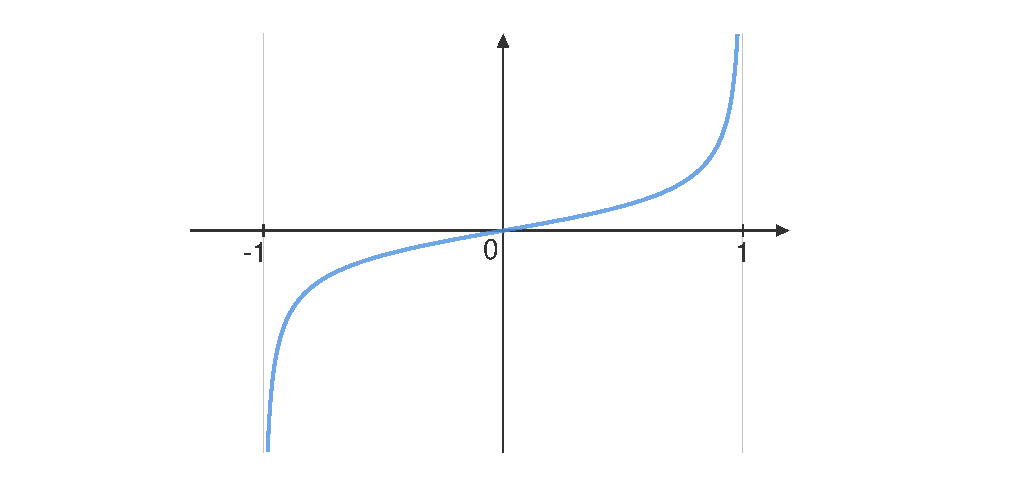
\includegraphics[trim={3cm 0 3cm 0},clip,width=\textwidth]{figs/rd_diffeomorphism.pdf}
\end{minipage}
we can pull back a rapidly decreasing form $\omega\in \Omega_{rd}^*(E)$ to 
$\Omega_{cv}^*(E)$ which is supported on the unit ball bundle. 
Note that the Schwartz property guarantees that $h^*\omega$ is smooth, i.e. 
all derivatives approach zero as $y \to 1$ since $\omega$ decays faster than any
polynomial.


Let us first look at the construction on an oriented Euclidean vector bundle
$E\xrightarrow{\pi} M$ of rank $n$ over a point $M=\{x_0\}$. 
Given coordinates $x^1,\ldots,x^n$ on $E$ from the local trivialisation,
a Thom form $U\in \Omega^n_{rd}(E)$ can be defined as
\[
	U(x) = (2\pi)^{-n/2}e^{-\abs{x}^2 /2} dx^1\wedge \ldots\wedge dx^n
\] 
Given the basis $e_1,\ldots,e_n$ of  $V$ corresponding to the coordinates
$x^1,\ldots,x^n$, denote the map $dx = dx^k \otimes e_k \in 
\Omega^1(E, V)$. Then $e^{-idx}\in \Omega(E,\bigwedge V)$ by taking a formal sum
of wedge products.
We can express this form in terms of the Berezin integral,
considered as a map $\int^B := \int \odif{e_1}\cdots\odif{e_n} 
: \Omega^*(E,\bigwedge V) \to \Omega^*(E)$.

\begin{lem} \label{lem:gaussian_integral} %1.49 BGV
	The form $U\in \Omega^n_{cv}(E)$ equals 
	\[
		 U(x) = (2\pi)^{-n/2} e^{-\abs{x}^2 /2} \epsilon(n)\int^B e^{-idx}
	\] 
	where $\epsilon(n)=1$ if  $n$ is even, otherwise  $i$.
\end{lem}
\begin{proof}
	The Berezin integral kills any forms of order less than $n$, so only
	multiples of $e_1 \wedge \ldots\wedge e_n$ remain.
	Hence,
	\begin{align*}
		\int^B e^{-idx} 
		&= (-i)^n \frac{1}{n!}\int^B (dx^k\otimes e_k)^n \\
		&= (-i)^n \int^B (dx^1\otimes e_1) \ldots(dx^n\otimes e_n) \\
		&= (-i)^n(-1)^{n(n-1)/2} \int^B dx^1\wedge \ldots\wedge dx^n\otimes e_1 \wedge\ldots\wedge e_n \\
		&= (-i)^n(-1)^{n(n-1)/2} dx^1\wedge \ldots\wedge dx^n
	\end{align*}
	Multiplication of elements of $\Omega(E,\bigwedge V)$ occur in
	the graded tensor product, so that this is a graded algebra. 
	In the second line, we have permuted all $n!$ terms into standard order, and
	terms of degree two commute.
	In the third line, $dx^i$ are separated from the  $e_i$, which
	anti-commute due to  $\Omega(E,\bigwedge V)$ being a graded algebra. 
	The lemma now follows, since
	$(-i)^n(-1)^{n(n-1)/2}$ equals 1 if $n$ is even, and otherwise  $-i$. 
\end{proof}
We will define the Thom form on a more general manifold by modification of the
above lemma. Denote $x \in \Omega^0(E,\pi^*E)$ as the \underline{tautological
section}, defined by $e\in E_p \mapsto e\in (\pi^*E)_{e} = E_{p}$.
Then choosing a Euclidean connection $\nabla^E$ on  $E$, we may replace  $dx$ by 
$\nabla^{\pi^*E} x \in \Omega^1(E,\pi^*E)$.

\begin{prop} \label{prop:derivative_berezin} %1.50 BGV
	If $\nabla$ is a metric connection on  $E$, this induces a covariant
	derivative on $\bigwedge E$. Then for any
	$\alpha\in\Omega(M,\bigwedge E)$, we have 
	\[
	d\int^B \alpha = \int^B \nabla\alpha
	\] 
\end{prop}
\begin{proof} 
	Given a non-vanishing section $\nu\in \Omega^1(M,\bigwedge^nE)$,
	the Berezin integral is given by the induced inner product on $\bigwedge E$
	with  $\nu$. Then  $\nabla$ induced on  $\bigwedge E$ is compatible with
	this inner product, and 
	\[
	d\gen{\nu,\omega} = \gen{\nabla \nu, \omega} + \gen{\nu, \nabla \omega}
	=\int^B \nabla\omega
	\] 
	where we have used the fact that $\nabla \nu = 0$, by definition of the
	Berezin integral on an oriented vector bundle with a metric connection.
\end{proof}

We will apply this proposition to the pullback vector bundle $\pi^*E \to E$, 
with induced connection $\nabla^{\pi^*E}=\pi^*\nabla^E$. Denote $V=\pi^*E$ to
simplify notation.
Let $\iota(s):\Omega^i(E,\bigwedge^j V) \to
\Omega^i(E,\bigwedge^{j-1} V)$ for $s\in\Gamma(V)$ be a contraction operator
defined in a similar fashion as \ref{def:contraction}, by the following
properties:
\begin{enumerate}[(1)]
    \item If $w\in \Omega^0(E,V)$, then  $\iota(s)w = \gen{s,w}$
	\item If $\alpha\in\Omega^i(E,\bigwedge^jV),
		\beta\in\Omega^k(E,\bigwedge^lV)$, then 
	 \[
	\iota(x)(\alpha\wedge \beta) 
	= (\iota(x)\alpha)\wedge\beta + (-1)^{i+j}\alpha\wedge(\iota(x)\beta)
	\] 
\end{enumerate}
Note that this uniquely defines $\iota(s)$ because the formulas can be applied
to a basis of $\bigwedge^iT^*E\otimes \bigwedge^jV$.

Denote $\nabla = \nabla^{\pi^*E}$. 
Recall that the curvature is a form in $\Omega^2(E,\End(V))$ 
which is skew-symmetric valued. We can identify $\mathfrak{so}(V)$ with 
$\bigwedge^2 V$ in the following way:
\begin{equation} \label{eq:so_wedge}
	A\in \mathfrak{so}(V) \mapsto \sum_{i<j} \gen{Ae_i,e_j} e_i\wedge e_j
\end{equation}
given a frame of $V$. Hence, we denote the curvature form as $F \in
\Omega^2(E,\bigwedge^2V)$.

\begin{prop} \label{prop:closed_prop} % 1.51 BGV
	Let $x \in \Omega^0(V)$ be the tautological section on $E$, and $\nabla$ the
	induced connection on $\bigwedge V$.
	Let $\omega_t = \frac{1}{2}t^2\abs{x}^2 + it\nabla x + F 
	\in \Omega(E,\bigwedge V)$. Then 
	\[
		(\nabla - it\iota(x))\omega_t = 0
	\] 
\end{prop}
\begin{proof}
	 By metric compatibility,
	$\nabla \abs{x}^2 = 2\gen{\nabla x, x} = -2\iota(x)\nabla x$.
	Next, we have $\nabla(\nabla x) = \iota(x) F$.
	Finally by Bianchi's identity, $\nabla F = 0$. Combining this,
	\[
	\nabla \omega_t = -t^2\iota(x) \nabla x + it\iota(x)F 
	\] 
	On the other hand, $\iota(x)\abs{x}^2 = 0$ by definition of $\iota(x)$, so
	\[
	it\iota(x)\omega_t = -t^2\iota(x) \nabla x + it\iota(x)F
	\] 
\end{proof}

We now define the Mathai-Quillen Thom form 
\begin{equation}
	U = (2\pi)^{-n/2}\epsilon(N) \int^B e^{-\frac{1}{2}\abs{x}^2-i\nabla x - F} \in \Omega^n(E)
\end{equation}
and its parameterised version $U_t = (2\pi)^{-n/2}\epsilon(N) \int^B e^{-\omega_t} \in
\Omega^n(E)$. To justify why $U_t\in\Omega^n(E)$, note that
$\omega_t\in\bigoplus_{i=0}^2 \Omega^i(E,\bigwedge^iV)$, and hence 
$e^{-\omega_t} \in \bigoplus_{i=0}^n \Omega^i(E,\bigwedge^iV)$. The Berezin
integral then only retains the top degree part. 

\begin{thm}
	The Mathai-Quillen form $U \in \Omega^n_{rd}(E)$ is a Thom form. 
\end{thm}
\begin{proof}
	% BGV Lemma 1.51
	We need to show that $U$ is closed, and integration along the fiber gives $1\in
	\Omega^0(E)$.
	From equation (\ref{eq:grassman_exp}), the exponential of $-\omega_t$
	can be written 
	\begin{equation} \label{eq:MQ_exp}
		e^{-\omega_t} = \sum_{k=0}^{n} \frac{e^{-t^2\abs{x}^2 /2}}{k!} (-it\nabla x
		- F)^k 
		= \sum_{k=0}^{\infty} \frac{1}{k!} (-\omega_t)^k
	\end{equation}
	Since $\nabla - it\iota(x)$ is an antiderivation, it follows from
	Proposition \ref{prop:closed_prop} that $(\nabla-it\iota(x)) e^{-\omega_t} =
	0$. 
	We can extend Proposition \ref{prop:derivative_berezin} to 
	$d\int^B\alpha = \int^B (\nabla-it\iota(s))\alpha$ for any	
	$\alpha\in\Omega(\bigwedge V)$ since $\iota(s)\alpha$ has no component in 
	the top exterior power.	
	Therefore it follows that $U_t \propto \int^B e^{-\omega_t}$ is closed.
	
	% BGV prop 1.52 says integral reduces to the case where $M$ is a point
	% Proof is found from Blau 
	From equation (\ref{eq:MQ_exp}), we can write the Thom form as 
	\[
	U_t = (2\pi)^{-n/2}\epsilon(N) e^{-\frac{1}{2}\abs{x}^2}\int^B e^{-i\nabla x -F}
	\] 
	To integrate $U_t \in \Omega(E)$ along the fiber of $V=\pi^*E$, we extract from
	the Berezin integral the part which is a $n$-form on the fiber of $V$,
	\begin{align*}
		\int_E (2\pi)^{-n/2}\epsilon(N) e^{-\frac{1}{2}\abs{x}^2}\int^B e^{-i\nabla x -F}
		&= (2\pi)^{-n/2}\epsilon(N) \int_E e^{-\frac{1}{2}\abs{x}^2}\int^B 
		e^{-idx}
		= 1 
	\end{align*}
	we are only left with the $dx$ term because the induced connection and
	curvature forms on  $\pi^*E$ do not have any components along the fiber.
	We have evaluated the integral using Lemma \ref{lem:gaussian_integral}.
\end{proof}

%%%%%%%%%%%%%%%%%%%%%%%%%%%%%%%
\begin{comment} % Blau approach
Let $E=P\times_\rho V$ be the associated bundle to $P$ with rank $2m$. 
basic forms on $P\times V$ are in correspondence with forms on  $E$.

A representative for the Thom class, called the Mathai-Quillen Thom form, is
given by
\begin{equation} \label{eq:mathai_quillen}
\Phi_\nabla(E) = \frac{1}{(2\pi)^m} e^{-v_a^2/2} \int \odif{\chi} 
\exp(\chi_a\Omega^{ab}\chi_b /2 + i\nabla v^a \chi_a)
\end{equation}
where $v^a \in \Omega^0(P\times V)$ are coordinates on $V$, and $\nabla v^a \in
\Omega^1(P\times V)$ is the exterior covariant derivative of $v^a$.
Not well defined globally, since using trivialisation to use coordinates? 

We claim that this defines a basic form in $\Omega^{2m}_\rho(P\times V)$,
and that it is a representative of the Thom class. 

To show that it is a basic form, we need to prove it is horizontal and $\rho$
equivariant.  

To show that is is a representative of the Thom class, we need to prove it is
closed and satisfies  $\pi^*\Phi_\nabla(E) = 1$.

Pullback by zero section is Pfaffian.
\end{comment} 
%%%%%%%%%%%%%%%%%%%%%%%%%%%%%%%

\begin{prop} % prop 1.53 BGV
	We have the transgression formula
	\[
	\odv{}{t} U_t = -i\epsilon(N) d\int^B x e^{-\omega_t}
	\] 
\end{prop}
\begin{prop} \label{prop:thom_pullback}
	Let $s\in \Gamma(M,E)$ be a section of $E$.
	The cohomology class of the pullback $s^*\Phi_\nabla(E) \in \Omega^{n}(M)$
	is independent of the section  $s\in\Gamma(E)$.
\end{prop}
\begin{proof}
	Integrating the transgression formula above from 0 to 1, 
	\[
		U_1 - U_0 = -id\int_0^1\int^B x e^{-t^2\abs{x}^2/2 +
		it\nabla x + F} \odif{t}
	\] 
	Note that $s^*U_0 = \epsilon(n)\int^B e^{-s^*F} \in \Omega(M)$. Since $F$ is
	the pullback curvature on $V = \pi^*E$, it is constant on 
	(why is $s^*U$ equal to the Pfaffian? use basis of V).

	Taking the pullback by $s$ on both sides, we find that $s^*U_1$ is
	cohomologous to the Euler class for any section $s$:  
	\[
		s^*U_1 - s^*U_0 = -id\int_0^1\int^B s\wedge e^{-t^2\abs{s}^2/2 +
		it\nabla s + F} \odif{t}
	\] 
	% TODO: complete proof
\end{proof}



\section{Universal Mathai-Quillen formula}
\begin{prop}
	Let $E\to M$ be an oriented vector bundle with fiber $V=\mathbb{R}^n$ 
	and  $P=\Fr_{\SO}(E)$ be the
	principal $\SO(n)$-bundle of orthonormal oriented frames on  $E$. Then 
	$P\times_{\SO(n)} V$ is canonically isomorphic to $E$ as a vector bundle. 
\end{prop} 
\begin{proof}
	The action of $A\in\SO(n)$ on $P\times V$ is 
	$
		([v_1 \cdots v_n], v) \cdot A = ([v_1 \cdots v_n] A, A^{-1} v) 
	$.
	Then the canonical isomorphism $\psi : P\times_{\SO(n)} V \to E$ is defined by
	\[
		[[v_1 \cdots v_n], v] \mapsto [v_1 \cdots v_n] v
	\] 
	It is clear that this is well defined, linear, smooth and preserves the
	fiber. The map is injective because $v_1,\ldots,v_n$ must be linearly
	independent, and surjective because $v_1,\ldots,v_n$ is a basis for $E_x$.
\end{proof}
% p104 MQformula
% cordes pg 103
Let $E\to M$ be an oriented vector bunde or rank  $n$ with a
metric and compatible connection, and fiber $V$. 
Then $E$ can be identified as the associated bundle $\Fr_{\SO}(E)\times_{\SO} V$ 
with the induced connection. 

More generally, consider a connected Lie group $G$ and 
principal $G$-bundle  $P\to M$ over a manifold of
dimension $n$ with a connection $\omega$. Let $\rho : G \to \SO(V)$ be a 
representation of rank $n$ (same as $\dim M$). 
This determines the associated vector bundle  $E:=P\times_\rho V \to M$
with typical fiber $V$. 

% Sources for this:
% naber p113
% guillemin 7.2, ch10
% constantinescu 2.2
Let $p_1,p_2$ be the projection maps from $P\times V$ to  $P$ and  $V$
respectively. Note that both maps are $G$-equivariant, where 
$V$ is considered as a $G$-manifold with action $v\cdot g = \rho(g)^{-1} v$.
The principal bundle $P\times V \to P\times_\rho V$ has the connection 
$p_1^*\omega$ (the reader should check this is a valid connection).
The Cartan map associated to this 
connection gives the homomorphism
\[
	\Omega_G(V) \xrightarrow{p_2^*} \Omega_G(P\times V) 
	\xrightarrow{\operatorname{Car}_{\omega}} \Omega(P\times V)_{bas}\simeq
	\Omega(E)
\] 
given by $\alpha \mapsto \operatorname{Hor}_{\omega}((p_2^*\alpha)(\Omega))$. 
Since  $P\times V \to E$ is a principal bundle,
$\Omega^*(E)\simeq \Omega^*(P\times V)_{bas}$ by definition of basic forms on a
principal bundle.

\begin{comment}
% as a composition with inclusion in top row
% https://q.uiver.app/#q=WzAsNyxbMSwwLCJXKFxcbWF0aGZyYWt7Z30pXFxvdGltZXNcXE9tZWdhKFYpIl0sWzMsMCwiXFxPbWVnYShQXFx0aW1lcyBWKSJdLFsxLDEsIihXKFxcbWF0aGZyYWt7Z30pXFxvdGltZXNcXE9tZWdhKFYpKV97YmFzfSJdLFszLDEsIlxcT21lZ2EoUFxcdGltZXMgVilfe2Jhc30iXSxbNCwxLCJcXHNpbWVxXFxPbWVnYShFKSJdLFswLDEsIlxcT21lZ2FfRyhWKVxcc2ltZXEiXSxbMiwwLCJcXE9tZWdhKFApXFxvdGltZXNcXE9tZWdhKFYpIl0sWzAsMl0sWzEsM10sWzIsMywiXFxvdmVybGluZXt3fSJdLFswLDYsInciXSxbNiwxLCIiLDAseyJzdHlsZSI6eyJ0YWlsIjp7Im5hbWUiOiJob29rIiwic2lkZSI6InRvcCJ9fX1dXQ==
\[\begin{tikzcd}[column sep=1em]
		&[-18pt] {W(\mathfrak{g})\otimes\Omega(V)} & {\Omega(P)\otimes\Omega(V)} 
		& {\Omega(P\times V)} \\
	{\Omega_G(V)\simeq} &[-18pt] {(W(\mathfrak{g})\otimes\Omega(V))_{bas}} &&
	{\Omega(P\times V)_{bas}} &[-18pt] {\simeq\Omega(E)}
				\arrow[from=1-2, to=2-2]
					\arrow[from=1-4, to=2-4]
						\arrow["{\overline{w}}", from=2-2, to=2-4]
							\arrow["w", from=1-2, to=1-3]
								\arrow["i",hook, from=1-3, to=1-4]
\end{tikzcd}\]

A few remarks are necessary to explain the diagram.
\begin{itemize}
\item 
The injection $i:\Omega(P)\otimes\Omega(V) \to \Omega(P\times V)$ can be defined
as follows. Denote by $p_1 : P\times V \to P$ and $p_2:P\times V \to V$ the 
canonical projections. Then the map is defined by $\omega \otimes \alpha
\mapsto p_1^*\omega \wedge p_2^*\alpha$.  

\item 
Since $w$ is a  $\mathfrak{g}$-dga morphism, so is  
$w:\Omega(\mathfrak{g})\otimes\Omega(V)\to \Omega(P)\otimes\Omega(V)$ because it
is the identity on  $\Omega(V)$. We claim that $i$ is also a $\mathfrak{g}$-dga morphism. 
\begin{itemize}
	\item Graded algebra homomorphism. It is linear by construction. It also respects
		multiplication because 
	\begin{align*}
		i((\omega_1\otimes\alpha_1)(\omega_2\otimes\alpha_2))
		&= i((-1)^{\abs{\alpha_1}\abs{\omega_2}}
		(\omega_1\wedge\omega_2)\otimes(\alpha_1\wedge \alpha_2)) \\
		&= (-1)^{\abs{\alpha_1}\abs{\omega_2}}
		p_1^*(\omega_1\wedge\omega_2)\wedge p_2^*(\alpha_1\wedge \alpha_2) \\
		&= (-1)^{\abs{\alpha_1}\abs{\omega_2}}p_1^*\omega_1\wedge
		p_1^*\omega_2\wedge p_2^*\alpha_1\wedge p_2^*\alpha_2  \\
		&= p_1^*\omega_1\wedge p_2^*\alpha_1 \wedge p_1^*\omega_2\wedge p_2^*\alpha_2 \\
		&= i(\omega_1\otimes \alpha_1)\wedge i(\omega_2\otimes \alpha_2) 
	\end{align*}
	\item Commutes with $d$ and $\iota_X$. This follows from by expanding the
		definitions of $d$ and  $\iota_X$ on the tensor product, given in
		equations (\ref{eq:tensor_ops}), and the fact that the pullbacks
		$p_1^*$ and $p_2^*$ commute with  $d$ and $\iota_X$.
\end{itemize}
Therefore, $w \circ i$ is a $\mathfrak{g}$-dga morphism and descends to the map
 $\overline{w}$ on the basic subcomplexes.
\end{itemize}
\end{comment}

% def depends on next proposition
\begin{defn} 
	An element $U\in (S(\g^*)\otimes \Omega(V))^G$ is a
	\underline{universal Thom form} if for any principal $G$-bundle $P\to M$ 
	with a connection, a representation $\rho : G\to \SO(V)$ and oriented
	associated bundle $P\times_\rho V$, the
	Cartan map $\operatorname{Car}_{\omega} : \Omega_{G}(V) \to
	\Omega(P\times_\rho V)$
	carries $U$ to a form representing the Thom class of $P\times_\rho V$.

	\begin{comment}
	A form $U\in (S(\so(V)^*)\otimes \Omega_{cv}(V))^G$ is a
	\underline{universal Thom form} if for any oriented vector
	bundle $E$ of rank $n$ with a metric and compatible connection, the 
	Cartan map $\operatorname{Car}_{\omega} : \Omega_{\SO(V)}(V) \to \Omega(E)$
	carries $U$ to a form representing the Thom class of $E$.
	\end{comment}
\end{defn} 

The integral over $V$ for equivariant forms
is a map  $\int_V : S(\g^*)\otimes \Omega(V) \to S(\g^*)$ defined by 
$\paren{\int_V \alpha}(X) = \int_V \alpha(X)$, where elements of $S(\g^*)$ are 
viewed as  polynomials on $\g$. 

\begin{thm} 
	A differential form $U\in (S(\mathfrak{g}^*)\otimes \Omega(V))^G$ is a 
	universal Thom form if and only if $U$ is closed and  $\int_V U = 1$.
\end{thm}
\begin{proof}
	Assume we have the same objects as above.
	When we pull back the form on $\Omega(V)$ to $\Omega(P\times V)$, it
	will still be a basic element because the projection $p_2$ is 
	$G$-equivariant. Next, the image of    
	$w:(S(\g)^*\otimes \Omega(P\times V))^G \to \Omega(P\times V)_{inv}$ 
	will be closed because the Weil homomorphism
	commutes with the differential operators. Finally, its horizontal
	projection is also closed. The same argument
	in reverse proves that $U$ must be closed if  $\Car_\omega(p_2^*U))$ is
	closed.

	% guillemin p157
	It remains to check that integration along the fiber of
	$\tau:=\operatorname{Car}_{\omega}(p_2^*U)\in\Omega(E)$ equals the integral
	over  $V$ of the universal Thom form.
	Fix a point $x_0\in M$, let $P_0=\pi^{-1}(x_0)$ be the fiber over $x_0$
	and $E_0$ be the fiber of $E$ over  $x_0$. 
	The fiber integral of $\tau$ only depends on the value of $\tau$ at the
	tangent space of the fiber submanifold, i.e. in the vertical direction (see
	figure ???). 
	So to evaluate the fiber integral at any point in $E_0$, it suffices to 
	consider the restriction to the principal $G$-bundle 
	$P_0\times V \to E_0$.

	The tangent space at $(p,v)\in P_0\times V$ 
	is $V_pP \oplus V$. But the connection on $P\times V$ is the pullback 
	$p_1^*\omega$, which is constant in the $V$ direction, and the curvature
	form vanishes on  $V_pP\oplus V$ since it is also a horizontal form. 
	If $\alpha_1,\ldots,\alpha_d$ is a dual basis for
	$\g^*$, the element $p_2^*U$ is a sum of terms of the form 
	$\beta_I \alpha_I$, where  $\beta_I \in \Omega(P\times V)$ are invariant
	forms. 
	After we replace the $\alpha_i$ by the curvature forms  $\Omega_i$, as a
	form on $P_0\times V$ we are only left with the term $\beta_0$. 
	Then taking the horizontal component amounts to only evaluating tangent
	vectors in $V$ at each point $(p,v)\in P_0\times V$ (see figure ???). 
	Subsequently, the fiber integral is the same as the integral of 
	$\beta_0$ over $V$, which equals 1 because $\int_V U = 1$.  
	% TODO draw diagram showing fiber integral, submanifold, horizontal proj
	\begin{comment} % first attempt
	This is defined on $\Omega(P\times_G V)\simeq \Omega(E)$ in exactly the same
	way, since coordinate functions on $E$ can be pulled back via the canonical
	isomorphism to coordinate functions on $P\times_G V$. 
	Recall that a local trivialisation 
	$\phi_\alpha : E|_{U_\alpha} \to U_\alpha \times
	\mathbb{R}^n$ gives coordinate functions $[t_1\cdots t_n] = p_2\phi_\alpha
	\in \mathbb{R}^n$ where $p_2$ is the projection on to $\mathbb{R}^n$.  
	This can be identified with coordinate functions on the associated bundle
	$[x_1\cdots]$
	\end{comment}
\end{proof}

The above theorem is proved in chapter 10 of \cite{guillemin} in the more
general context of a $K$-manifold $E=P\times_\rho V$, and a principal
$G$-bundle  $P\times V \to P\times_\rho V$, with associated Cartan map
$\Car_\omega : \Omega_{G\times K}(P\times V)\to\Omega_K(E)$. The Thom form is
obtained from the map $\Car_{\omega}(p_2^*U)$ where $U\in\Omega_{G\times K}(V)$.

% Guillemin 7.2
We shall now construct the Mathai-Quillen universal Thom form.
Let $V$ be a real vector space with standard inner product, and $\rho : G \to
\SO(V)$ be a rep of the Lie group $G$, with induced rep $\rho_* :
\mathfrak{g}\to \so(V)$.
We will apply the Berezin integral to a form in $S(\mathfrak{g}^*)\otimes 
\Omega(V) \otimes \bigwedge V$. 
Fix an oriented orthonormal basis $\{e_1,\ldots,e_n\}$ for
$V$, which allows us to define the Berezin integral, with corresponding
coordinate functions $x_1,\ldots,x_n$.   
Let  $\{X_1,\ldots,X_m\}$ be a basis of $\mathfrak{so}(V)$, with corresponding
dual basis $\{u_1,\ldots,u_m\}$ where $m= \frac{1}{2}n(n-1)$. Recall that we 
can identify $\mathfrak{so}(V)$ with 
$\bigwedge^2 V$ via equation (\ref{eq:so_wedge}), restated here 
\[
	X_a \in\mathfrak{so}(V) \mapsto \sum_{i<j}\gen{X_a e_i,e_j} e_i\wedge e_j
	= \frac{1}{2}\sum_{i} e_i\wedge X_a e_i
\] 
Denote $dx := \sum_i dx_i \otimes e_i \in \Omega^1(V)\otimes V$. Define the element 
\begin{equation} % 7.16 guillemin % cordes eq 11.13 % naber 3.18
	\label{eq:universal_thom_exponent}
	\sigma := -\frac{1}{2}\abs{x}^2 - idx 
	- \sum_a u_a\rho_* \otimes X_a 
	\quad \in S(\g^*) \otimes \Omega(V) \otimes \bigwedge V
\end{equation}
which is analogous to $\omega_1$ as defined in Prop \ref{prop:closed_prop}.
Note that $u_a \rho_* \in \mathfrak{g}^*$.
In components, if $M^a = [\gen{ X_ae_i,e_j}]_{ji}$, we can write the same
element as 
\begin{equation} \label{eq:universal_thom_exponent2}
\sigma = -\frac{1}{2}\abs{x}^2 - i\sum_i dx_i\otimes e_i 
	-\frac{1}{2} \sum_{i,j} (\rho_*)_{ji}e_i\wedge e_j
\end{equation}
since $u_aX_a$ is the identity on  $\so(V)$, and $(\rho_*)_{ji} \in \mathfrak{g}^*$.
Consider its Berezin integral
\begin{equation} \label{eq:universal_thom}
	U := \epsilon(n)(2\pi)^{-n /2}\int^B \exp\paren{\sigma}  
	\quad\in S(\g^*)\otimes \Omega(V)
\end{equation}
where $\epsilon(n)=1$ if $n$ is even and otherwise $\epsilon(n)=i$.

\begin{thm} \label{thm:uinversal_Thom}
	The element $U \in S(\mathfrak{g}^*) \otimes \Omega(V)$ defined above  
	is a universal Thom form.
\end{thm}
\begin{proof} % Guillemin p86-87
We need to show that it is invariant and
equivariantly closed in the Cartan model, and integration along the
fiber gives 1. 


(1) Closed. 
We can consider the Cartan
differential $\delta_C = d - \sum u_k\iota_k$ as an operator on 
$S(\so(V)^*)\otimes\Omega(V)\otimes\bigwedge V$ by acting trivially on
the last factor, so that it commutes with the Berezin integral. 
It suffices to show $U$ is closed as a form on  $S(\so(V)^*)\otimes \Omega(V)$,
because the map  $\rho^* : S(\so(V)^*)\to S(\g^*)$ given by  $u_i\mapsto
u_i\circ \rho_*$ commutes with the Cartan differential. This can be seen most
easily by viewing the elements as polynomials as in Theorem
\ref{thm:cartan_diff}, which shows that  $(\delta_C \rho_* \alpha)(X) 
= (\rho_*\delta_C \alpha)(\rho(X)) = (d-\iota_{\rho(X)})\alpha(\rho(X))$, noting
that $\iota_X$ and  $\iota_{\rho(X)}$ act the same way on $\Omega(V)$.

For the first term, only $d$ acts to give $\delta_C \abs{x}^2 = 2x_i dx_i$.
On the second term, $d^2=0$ and we need to evaluate $u_a\iota_a dx_i$. 
Since $x_i$ projects to the $i$th component of a vector in $V$, and the action
of $e^{tX_k}$ is matrix multiplication, for $v\in V$ in the tangent space
\begin{align} \label{eq:interior_dx}
	\iota_a dx_i(v)
	= d x_i \paren{\odv{}{t}_{t=0} e^{-tX_a} v} 
	= -x_i \paren{X_a v} 
\end{align}
Hence, $u_a\iota_a dx_i = -u_a\otimes x_i \circ X_a$. The third term is a
multiple of $u_i$ and constant on $\Omega(V)$,
hence maps to zero by  $\delta_C$. Thus, 
\begin{align}
	(d-u_a\iota_a) \sigma 
&= -x_i dx_i - u_a \otimes i x_iX_a \otimes e_i \nonumber \\
&= -x_i dx_i - u_a \otimes i x_j \otimes X_a e_j 
\end{align}
which is justified by $x_j$ being the coordinate functions of $e_j$:
\begin{equation} \label{eq:move_operator_tensor}
x_i X_a \otimes e_i 
= \gen{X_ae_j,e_i}x_j \otimes e_i 
= x_j \otimes \gen{X_ae_j,e_i}e_i 
= x_j \otimes X_a e_j 
\end{equation}
The key observation is that $\delta_C$ acts by lowering the degree of the
$\bigwedge V$ part. More precisely, consider the action of the Berezin
derivative/integral
\begin{align*}
\pdv{}{e_k} \paren{-\sum_{i<j} u_a\otimes e_i\wedge M^a_{ji}e_j}
&= -\sum_{i>k} u_a\otimes M^a_{ik}e_i + 
 \sum_{i<k} u_a\otimes M^a_{ki}e_i \\
&= -\sum_{i} u_a\otimes M^a_{ik}e_i  
= -u_a\otimes X_a e_k  
\end{align*}
since $M^a_{ij}=-M^a_{ji}$. Applying $\pdv{}{e_k}$ to the other term,
\[
\pdv{}{e_k} (-idx_i \otimes e_i) = idx_k
\] 
because $e_i$ anti-commutes with  $dx_i$. We have shown that
\begin{equation}
\delta_C \sigma = \paren{\sum_{k} ix_k \pdv{}{e_k}}\sigma
\end{equation}
It follows that this also holds for $\exp (\sigma)$, because  $\delta_C$ is an
anti-derivation. Therefore, 
\[
\delta_C \int^B \exp(\sigma) 
= \int^B \delta_C \exp(\sigma)
= \int^B ix_k \pdv{}{e_k} \exp(\sigma) = 0
\] 
as the Berezin derivative kills any top degree terms in $\bigwedge V$.

(2) Integral along the fiber. We need to extract the coefficient of $dx_1\wedge
\ldots\wedge dx_n$. Therefore, the last term in $\sigma$ does not contribute,
and 
 \[
	 \int_V U = \epsilon(n)(2\pi)^{-n /2}\int_V e^{-\abs{x}^2} \int^B \exp(-idx_k \otimes e_k) 
\] 
But we know $\int^Be^{-idx_k\otimes e_k}$ evaluates to 
$(-i)^n(-1)^{n(n-1)/2} dx_1\wedge \ldots\wedge dx_n$ by Lemma
\ref{lem:gaussian_integral}. Hence, the integral of $U$ along the fiber $V$ is 1.

(3) Invariant. % proved in p27 Constantinecu PhD
It suffices to show the terms in $\sigma$ are invariant, because
the Lie derivative is a derivation. We can extend the action of $G$ to the
graded algebra $S(\g^*)\otimes \Omega(V)\otimes \bigwedge V$,
acting on the $\bigwedge V$ component by multiplication by $\rho(g)^{-1}$. 
Note that the Berezin integral is
invariant under the action on $\bigwedge V$. This gives an associated Lie derivative,
corresponding to multiplication by $\rho_*(X)$ for  $X\in\mathfrak{g}$.

It is clear that $\abs{x}^2$ is invariant, because $\rho(g)$ has determinant 1.
Next, we show $dx_i\otimes e_i$ is invariant by applying $\mathcal{L}_X$,
\[
\mathcal{L}_X (dx_i\otimes e_i) = \iota_X(dx_i) \otimes e_i + dx_i \otimes
\rho_*(X)e_i = 0
\] 
by equations (\ref{eq:interior_dx}) and (\ref{eq:move_operator_tensor}).
Finally, to apply $\mathcal{L}_X$, recall that the action on $S(\g^*)$ 
is the coadjoint representation $\mathcal{L}_X \alpha(Y) = -\alpha ([X,Y])$. 
The action on $V$ is  $\mathcal{L}_X v = \rho_*(X)v$.
We can denote the third term in $\sigma$
as $\frac{1}{2}e_i\wedge (\rho_*)_{ji} e_j \in \g^*\otimes \bigwedge^2V$,
since $u_aX_a$ is just the identity.
For $X,Y\in\g$, with  $\rho_*(X)=A,\rho_*(Y)=B$,
\begin{align*}
	&\quad\;(\mathcal{L}_X(e_i \wedge (\rho_*)_{ji} e_j))(Y) \\
	&= (A e_i \wedge \rho_* e_i)(Y)
	- e_i \wedge \rho_*([X,Y]) e_i
	+ (e_i \wedge \rho_* A e_i)(Y) \\
	&= Ae_i \wedge B e_i
	- e_i \wedge (AB-BA) e_i
	+ e_i \wedge A Be_i \tag{$\star$} \\
	&= -e_i \wedge BA e_i
	- e_i \wedge (AB-BA) e_i
	+ e_i \wedge AB e_i = 0\tag{$\star\star$}
\end{align*}
where we begin by using the derivation property of $\mathcal{L}_X$, and explain
the next two lines below.

Proof of ($\star$): This step initially looks wrong, but recall that the term is
to be interpreted as 
\[
\sum_{i,j}e_i\wedge (\rho_*(Y))_{ji} (Ae_j)
=\sum_{i,j}e_i\wedge \sum_kB_{ji} A_{kj}e_k
=\sum_{i}e_i\wedge \sum_{k,j}A_{kj}B_{ji} e_k
=\sum_{i}e_i\wedge AB e_i
\] 
Proof of ($\star\star$): This is just an application of the more general property
\[
Ae_i \wedge Be_i
= A_{ji}e_j \wedge B_{ki}e_k
= e_j \wedge B_{ki}A^\intercal_{ij}e_k
= e_j \wedge BA^\intercal e_j 
\] 
Finally, $U$ is invariant because $\mathcal{L}_X$ commutes with the Berezin
integral.
\end{proof}

The proof of (1) closure is due to \citet{guillemin} and part of (3) invariance
is a corrected version of the proof in \citet[p.27]{constantinescu}. In
particular, the steps $(\star)$ and  $(\star\star)$ are corrected, as well as
the action of $\mathcal{L}_X$ on $\mathfrak{g}^*$. 

\begin{remark}
	The minus sign in $e^{-tX_a}$ in the fundamental vector field over $V$ in
	equation (\ref{eq:interior_dx}) arises due to the fact that the
	$\SO(V)$-action on $V$ is a right action. In general, this is so that the
	map $\g \to \Gamma(TM)$ is a Lie algebra homomorphism. 
\end{remark}	
 
% TODO prove equivalence to usual form
To relate our formula to other versions in literature, let $\chi =
(e_1,\ldots,e_n)$ be the Grassman variables for $V$. 
In more compact notation, the third term of $\sigma$ can be written  
as $\frac{1}{2} e_i \wedge (\rho_*)_{ij} e_j = \frac{1}{2} \chi^\intercal
(\rho_*) \chi$. Then the Mathai-Quillen Thom form 
$U\in S(\mathfrak{g}^*)\otimes \Omega(V)$ can be alternatively written as 
\begin{equation} \label{eq:universal_thom_form} % AJ 2.1
	U = \epsilon(n)(2\pi)^{-n /2}e^{-\abs{x}^2} 
	\int^B \exp \paren{\frac{1}{2}\chi^{\intercal}(\rho_*)\chi -
idx^{\intercal}\chi} \odif{\chi} 
\end{equation}
If $\rho_*(X)\in\so(V)$ is always invertible, we can apply
Proposition \ref{prop:berezin_formula}, to get
\[
	U = \epsilon(n)(2\pi)^{-n/2} \Pf(\rho_*) \exp(-\abs{x}^2-dx^{\intercal} (\rho_*)^{-1}dx)
\] 
We can also obtain a universal Thom form in the Weil model, by 
applying the Weil-Cartan isomorphism $(S(\mathfrak{g}^*)\otimes \Omega(V))^G
\xrightarrow{\simeq}(W(\mathfrak{g})\otimes \Omega(V))_{bas}$. 

\begin{comment} % Mathai-Quillen forms in Weil model 
\[% cordes eq11.12
		U = (2\pi)^{-m} \Pf(\phi) \exp(-\abs{x}^2-\gen{\nabla x,\phi^{-1}\nabla x})
\] 
\[%MQformula weil eq 6.2 (extended from 1.8)
	U = (2\pi)^{-m}\Pf(\Omega) \exp(-x^2-(dx+\theta x)^\intercal \Omega^{-1}
	(dx+\theta x))
\]
\end{comment}


\vspace{5mm}
\hrule 
\vspace{5mm}

\textbf{Bibliographical notes}
{\small
\begin{itemize}
	\item A more comprehensive treatment of the Thom isomorphism can be found in
		\citet{bott_tu}.  
	\item The Mathai-Quillen formula described in section
		\ref{section:mq_formula} is based on section 
		section 1.6 of \cite{bgv}.
	\item The book by \citet{guillemin} gives an exposition of the
	Mathai-Quillen formula in the equivariant case 
\end{itemize}
}

%\chapter{Donaldson-Witten theory in MQ formalism}
\label{chapter4}
% See AJ intro
In finite dimensions, the Mathai-Quillen formula gives an explicit differential
form representative of the Euler class. 
It was shown by Atiyah and
Jeffrey \cite{atiyahlagrangians} that not only can the zero dimensional
Donaldson invariant can be identified with the Euler number of a vector bundle
over $\mathcal{A} /\mathcal{G}$, but the Donaldson invariants in general can be
written as an integral of a Mathai-Quillen type form over the gauge equivalence
classes of irreducible connections, similar to (reference Gauss-Bonnet formula
with Mathai-Quillen).
Moreover, they have been able to reproduce Witten's
action functional from twisted SUSY YM theory term by term from purely geometric
considerations.

Conversely,
the Mathai-Quillen formalism makes it possible to construct a cohomological field
theory starting from a moduli problem.

\section{Thom analog for principal bundles}
Before we construct the Atiyah-Jeffrey formula, we first need to develop an
analog of the Thom form for a principal $G$-bundle $P\to M$. Assume $G$ is
compact with $\dim G = d, \dim M = n$. 
We wish to construct a differential form  $W\in \Omega^d(P)$
such that its integral along the fiber equals 1, so that by 
Proposition \ref{prop:projection_formula}, for all $\beta\in \Omega_c^B(P)$
\[
\int_M \beta = \int_P \pi^*\beta \wedge W
\] 
Of course, we will need an orientation on $M$ and $G$, which gives the local
product orientation on $P$.   

Denote by $\omega \in \Omega^1(P,\g)$ the connection on
$P$ induced by the metric on $P$ so that the horizontal and
vertical subspaces are orthogonal complements. Let $\eta_1,\ldots,\eta_d$ be an 
orthonormal basis for $\g$ consistent with the orientation on $G$.
We will show that
\begin{equation} \label{eq:principal_thom}
W := \int^B \exp(\omega) d\eta 
= \int^B \exp(\omega_a\eta_a) d\eta = \omega_1 \wedge \cdots \wedge\omega_d
\;\in \Omega^d(P\times V)
\end{equation}
is the desired vertical volume form. Multiplication inside the Berezin
integral occurs in the graded tensor product $\Omega(P)\otimes \g$, 
so $\omega_a\eta_a$ all have degree two.

The integral along the $G$-orbit 
$\pi_*:\Omega^{*}(P\times V) \to \Omega^{*-d}(P\times_G V)$ is defined as in 
section \ref{section:fiber_integration}, where the integral defined by 
pulling back to a form on $G$ via a trivialisation
$\psi:G\xrightarrow{\simeq} \pi^{-1}(x)$.   

% construct left invariant metric on $G$ first
We will now turn $G$ into Riemannian manifold by choosing a metric on $\g$, then
extend this metric to $T_gG$ via left translations. That is, define
$\gen{u,v}_g = \gen{DL_g^{-1}(u),DL_g^{-1}(v)}_e$ where $L_g(h) = gh$.
By construction, this is a left-invariant metric. In fact, because $G$ is
compact we can turn it into a
bi-invariant metric by Haar integrating the metric, but this is not needed.

\begin{prop}
	For all $p\in P$,  $L_p^* W \in \Omega^d(G)$ is equal to the unique
	Riemannian volume form induced by the left-invariant metric on $G$. 
\end{prop}
\begin{proof}
	Let $\epsilon_1,\ldots,\epsilon_d\in T^*_eG$ be the orthonormal coframe dual
	to $\eta_1,\ldots,\eta_d$. At a point $g\in G$, the tangent vectors are
	transported to  $DL_g \eta_i$ while the coframe is transported to 
	$\epsilon_i\circ DL_{g}^{-1} \in T^*_gG$, where $L_g$ is left multiplication
	by  $g$. Then the Riemannian volume form is given by
	\[
	    \epsilon_1\circ DL_{g}^{-1} \wedge \cdots\wedge \epsilon_d\circ DL_{g}^{-1}
	\] 
	The covectors are orthonormal because the metric is left invariant. 
	For $X\in \g$, the pullback
	by $L_p : G \to P_{\pi(p)}$ of $\theta := \omega_a \in \Omega^1(P)$ is
	\begin{align*}
		(L_p^*\theta)_g(DL_g X) 
		&= \theta_{p\cdot g}(DL_p \circ DL_g(X)) \\
		&= \theta_{p\cdot g}(DL_{p\cdot g} (X)) \\
		&= \theta_{p\cdot g}\paren{\odv{}{t}_{t=0} (p\cdot g \exp(tX))} \\
		&= \epsilon_a(X)
		= (\epsilon_a DL_g^{-1})DL_g(X)
	\end{align*}
	which shows that $L_p^*\omega_a = \epsilon_a\circ DL_g^{-1}$, so 
	\[
	L_p^* (\omega_1\wedge \cdots\omega_d)
	= \epsilon_1\circ DL_{g}^{-1} \wedge \cdots\wedge \epsilon_d\circ DL_{g}^{-1}
	\] 
	as required.
\end{proof}
normalised so that integral along the $G$-orbit $\pi_*W = 1$. 
\begin{cor}
	The integral along the fiber of $W$ is  $\pi^*W = 1 \in \Omega^0(G)$
\end{cor}
\begin{proof}
	Show that a trivialisation $\psi : G \to \pi^{-1}(b)$ is of the form of 
	$L_p : G \to \pi^{-1}(b)$ where $p= \Psi(e)$
\end{proof}




\section{Atiyah-Jeffrey formula}
This section derives another version of the Mathai-Quillen
Thom form, which will be then be formally applied to the Donaldson-Witten context. 
We consider the following setup: 
\begin{itemize}
	\item $G$ is a compact connected Lie group of dimension $d$
	\item $P\to M$ is a principal $G$-bundle  of dimension  $2m+d$.
	\item Choose an $\Ad$-invariant metric on $\g$ using Theorem 
		\ref{thm:lie_inner_product}
	\item Similarly, construct a metric on $P$ which is invariant under the 
		action of  $G$, by averaging any Riemannian metric on $P$ with respect 
		to a Haar measure  
	\item At each point $p\in P$, this Riemannian metric defines an orthogonal
complement to the vertical tangent space. Since these subspaces are invariant
under the action of $G$, this determines a connection  $\omega$ on  $P$.
Moving forward, we will solely use this connection.
	\item $V$ is a real vector space, with $\dim V = 2m$ and a
rep $\rho : G \to \SO(V)$
	\item $E:= P\times_G V$ is the associated vector bundle.
\end{itemize}

% AJ p124, Naber p123
Our starting point is the universal Mathai-Quillen formula
(equation \ref{eq:universal_thom_form}), an element in the
Cartan model $S(\mathfrak{g}^*)\otimes \Omega(V)$, restated here
\begin{equation} \label{eq:universal_thom_form2}
	U = (2\pi)^{-m}e^{-\abs{x}^2}\int^B
	\exp\paren{\frac{1}{2}\chi^{\intercal}\rho_*\chi - idx^\intercal \chi}
	\odif{\chi}
\end{equation}
where $\chi = (e_1,\ldots,e_{2m})$ is a basis for $V$.

\vspace{1ex}\noindent
\textbf{Manipulation 1: Replace $\Omega$ with  $d\omega$} \\
Recall that we can obtain a Thom form on $E$ via the Cartan map, which is given
by $\alpha\to \operatorname{Hor}(p_2^*\alpha(\Omega)) \in \Omega(P\times V)_{bas}$, 
where $p_2:P\times V\to V$ is the projection onto $V$.  
The curvature is related to the connection by 
$\Omega = d\omega + \frac{1}{2}[\omega\wedge \omega]$, but $\omega=0$ on
horizontal vectors (by definition of horizontal subspace). Since the Cartan map
then only evaluates on the horizontal projection of tangent vectors, we can 
replace  $\Omega$ by  $d\omega$ in the Cartan map. 

\vspace{1ex}\noindent
\textbf{Manipulation 2: Replace $d\omega$ with  $R^{-1}dC^*$} \\
Recall that $C_p : \mathfrak{g} \to V_pP$ defined by  $C_p(X) = \odv{}{t}_{t=0}
(p\cdot \exp(tX))$ is the canonical identification of the Lie algebra with the
vectical tangent space at $p\in P$. Both spaces are inner product vector spaces,
and hence $C_p$ has an adjoint  $C_p^* : T_pP \to \g$. For $X,Y\in \g$, it
satisfies 
\[
	\gen{C_p(X), C_p(Y)} = \gen[*]{C_p^*C_p(X),Y}_{\g} = \gen{R_p X, Y}_{\g}
\] 
where $R := C_p^*\circ C_p : \g \to \g$. It is clear that $R_p$ is self-adjoint
and an isomorphism since $C_p$ is an isomorphism. 
Also note that $C_p^*$ vanishes on horizontal vectors, as 
$\gen[*]{X,C_p^*(v)} = \gen{C_p(X),v}$ vanishes on
all horizontal $v\in T_p$ due to $C_p(X)\in V_pP$. 

If $\omega\in \Omega(P,\g)$ is 
the connection 1-form, then $\omega_p(X) = C_p^{-1}(X)$. Thus, we have the
pointwise matrix equation $C^* = R\omega$, or $\omega = R^{-1}C^*$. From this,
we compute its differential 
\[
d\omega = R^{-1} dC^* + dR^{-1} \wedge C^*
\] 
The last term vanishes on a pair of horizontal vectors, so again, we can replace
$d\omega$ with $R^{-1}dC^*$, since the Cartan map will only evaluate on the
horizontal vectors.


\vspace{1ex}\noindent
\textbf{Manipulation 3: Double Fourier transform to avoid inverting $R$} \\
The next objective is to remove the explicit inverse $R^{-1}$ by using the
Fourier inversion formula. Recall that the Fourier transform is an automorphism
of the Schwartz space on any vector space $W$. If  $dw\in\bigwedge^n W$ is a
volume element with corresponding dual volume element $dy\in \bigwedge^nW^*$,
then the Fourier inversion formula states that 
\[
	f(w) =
	(2\pi)^{-n}\int_{W^*}\int_{W}e^{i\gen{w,y}}e^{-i\gen{z,y}}f(z)\odif{z}\odif{y}
\] 
Note that for a real vector space the integral is the same if we multiply both
exponents by -1.
If we identify $W$ with  $W^*$ via some inner product, this becomes a double
integral over $W$. For a self-adjoint matrix $R$ with positive determinant, we
can compute  $f(R^{-1}w)$ by making the change of variables $w \to R^{-1}w$ and
$y\to Ry$, in which case $\gen{R^{-1}w,Ry}=\gen{w,y}$ and $d(Ry)=\det R dy$. 
The inversion formula becomes
\[
f(R^{-1}w) = (2\pi)^{-n}\iint_W e^{i\gen{w,y}}e^{-i\gen{z,Ry}}f(z)\det R\odif{z}\odif{y}
\] 
We now consider the universal Mathai-Quillen element as a $\Omega(V)$-valued 
function $f:\g \to \Omega(V)$ on the vector space $\g$, 
\[
f(X) = (2\pi)^{-m}e^{-\abs{x}^2}\int^B
	\exp\paren{\frac{1}{2}\chi^{\intercal}\rho_*(X)\chi - idx^\intercal \chi}
	\odif{\chi}
\] 
which we wish to
evaluate at $R^{-1}dC^* \in \Omega^2(P,\g)$. By the inversion formula above,
\begin{align} \label{eq:fourier_thom}
	f(R^{-1}dC^*) = (2\pi)^{-d-m}e^{-\abs{x}^2}\iint_{\g}\int^B 
	&\exp\Big(\frac{1}{2}\chi^{\intercal}\rho_*(X)\chi - idx^\intercal \chi\\
	&+i\gen{dC^*,\lambda}-i\gen{\phi,R\lambda}\Big) \det R
	\odif{\chi} \odif{\phi}\odif{\lambda} \nonumber
\end{align}
where $\lambda, \phi \in \g$ are Lie algebra variables. 
\begin{remark} % naber p126
	Note that the original function $f(X)$ is a polynomial in $X\in\g$, and
	therefore not in the Schwartz space. This can be made more precise by
	inserting a rapidly decaying test function $e^{-\epsilon\gen{X,X}}$ and
	taking the limit as $\epsilon\to 0$.
\end{remark}

\vspace{1ex}\noindent
\textbf{Manipulation 4: Horizontal projection via integration along $G$-orbits} \\
% naber p127
The final step is to take the horizontal projection of the invariant element in
$\Omega^{2m}(P\times V)$. 
The intuition is that taking the wedge product with the invariant 
volume form $W\in\Omega^d(P)$, which contains all vertical components, 
gives only terms which did not have a vertical part but now with a factor of 
$W$. After integrating out the vertical part of these terms,  
the result is the horizontal part of the original element in
$\Omega(P\times V)$.

% TODO prove this as a proposition

\section{Interpretation of Donaldson-Witten theory}
We can now apply the Atiyah-Jeffrey Thom form to the infinite dimensional
setting of Donaldson-Witten theory. 
The spaces we now consider are 
\begin{itemize}
	\item principal bundle $P$: space of irreducible connections  $\mathcal{A}$ 
		over a compact oriented 4-manifold $M$
	\item structure group $G$: group of bundle automorphisms  $\mathcal{G}$ 
	\item vector space $V$: self dual 2-forms $\Omega^{2,+}(\ad P)$ ??
	\item section $s:P\to V$: self-dual part of curvature  $s=-F^+$
\end{itemize}
Donaldson only treats the case $G=\SU(2)$ because of singularities in the moduli
space, however we do not worry about this (??). Since our objective is to apply the
formula to the infinite dimensional vector space $\Omega^{2,+}(\ad P)$, complete
rigor (for this particular application) is out of the question anyway. 

Although $e(E)$ and  $\int_X e(E)$ do not make sense for
infinite dimensional  $E$ and  $X$, the Mathai-Quillen form  $e_{s,\Delta}$ can
be used to formally define regularized Euler numbers $\chi_s(E) := \int_X
e_{s,\Delta}(E)$. Although not independent of $s$, these numbers  $\chi_s(E)$
are of topological interest for certain choices of  $s$.  


\section{TQFT as a generalisation of Mathai-Quillen}
% section 4.2 MQintro


\vspace{5mm}
\hrule 
\vspace{5mm}

\textbf{Bibliographical notes}
{\small
\begin{itemize}
	\item The lecture notes by \citet{cordes95} explores these topics from the
	from the perspective of physics, and how it relates to twisted
	$\mathcal{N}=2$ topological field theory.
	\item 
\end{itemize}
}



%etc




%APPENDICES


% change chapter name and counters (eg Chapter 1 -> Appendix A)
\appendix


% assuming there are files appendix1.tex etc...

\chapter{Reference Guide}
\label{appendix1}

\section{Reference Guide}
\cite{cernTQFT} is a 63 page introduction to TQFT, including the Mathai-Quillen
formalism and Donaldson Witten theory using twisted $N=2$ supersymmetry.
Lacking details

\cite{wittenTQFT} is the seminal article on twisted supersymmetric gauge theory.
Including how donaldson invariants arise

\cite{birminghamTFT} is a 366pg textbook on supersymmetry, BRST, euler
character, sigma models, donaldson theory, Schwarz type TFTs, topological
gravity and renormalization

\cite{cordes95} is 247pg of lecture notes, and focuses on equivariant cohomology
and TQFT from pg 75. Moves through topics very quickly.

\cite{axiomTQFTintro} Motivates the functorial axiomatisation of TQFT using the
path integral approach

\cite{marino} 40 pages, goes through Donaldson invariants, supersymmetry and donaldson
witten theory, by stating a number of result, but without detail and lacking
proofs. 

\cite{moore} 80 pg, similar to marino. Focuses on path integral approach to
cohomological TFT, and Mathai quillen

\cite{TQFTbook} More detailed version of marino's lectures on TFT. 

\cite{MQformula} is the original paper by Mathai and Quillen which introduced a
formula for the euler number.

\cite{atiyahlagrangians} a short article showing how Witten's Lagrangian should
be understood in terms on the Gauss-Bonnet formula. Starts with Mathai-Quillen
formula for Thom class

\cite{MQintro} is a 35 pg introductory accound of the previous paper, beginning
with Mathai-Quillen formalism for finite dimen vector bundles





%\chapter{Grassman Calculus} 
\label{appendix2}
% Most of this chapter is from Lecture 10: Fermions in the Grassman formalism
\begin{defn}
	Let $V$ be a complex or real vector space.
	A \underline{Grassman number} is an element $x\in
	\bigwedge(V)$ in the exterior algebra of $V$.
	Given a choice of basis $\{\theta_i\}_{i=1}^{\infty}$ for $V$, a
	\underline{Grassman variable} is an element of the basis set.

	The Grassman numbers are typically equipped with a linear involution operator
	$*$ that extends complex conjugation in the following way: for all
	$\lambda,\mu\in\mathbb{C}$	
	\[
	(\lambda x + \mu y)^* = \lambda^* x^* + \mu^*y^*,	\qquad
	\theta^* = \theta, \qquad
	(\theta_1\theta_2\cdots\theta_k)^*=\theta_k\cdots\theta_2\theta_1
	\] 
	where $\theta,\theta_1,\ldots,\theta_k$ are in the basis set, and $x,y$ are
	Grassman numbers.
\end{defn}

It is standard to omit the wedge symbol $\wedge$ when writing a Grassman number.
The Grassman numbers have a $\mathbb{Z}_2$-grading given by $\bigwedge(V) =
\bigwedge_+(V) \oplus \bigwedge_-(V)$ which are subspaces generated by products
of an even (resp. odd) number of Grassman variables. Elements in
$\bigwedge_-(V)$ anti-commute, so are called a-numbers, while elements in 
$\bigwedge_+(V)$ commute, so are called c-numbers.

\section{Differentiation}
Let $A\in \bigwedge(V)$. For a given Grassman variable  $\theta_i$, after some
commutations we can uniquely write $A = A_1 + \theta_iA_2$ where $A_1,A_2$ do not
contain $\theta_i$. Then the differential operator with respect to $\theta_i$ is
defined as
\[
\pdv{A}{\theta_i} = A_2
\] 
In particular, we have $\pdv{\theta_j}{\theta_i} = \delta_{ij}$.

Note that the action of $\pdv{}{\theta_i}$ consists of commuting $\theta_i$ to
the left in all monomials before suppressing it. So the
derivaive of a product does not satisfy the usual Leibnitz rule.

Let $P$ be the algebra automorphism which satisfies $P(\theta_i)=-\theta_i$ for
each Grassman variable. Note that this relation uniquely determines  $P$,
which has the properties
$P(\theta_{i_1}\cdots\theta_{i_p})=(-1)^p\theta_{i_1}\cdots\theta_{i_p}$ and  
$A\theta_i = \theta_iP(A)$.

We find that the Leibnitz rule is replaced by
 \[
\pdv{}{\theta_i}(AB) = \pdv{A}{\theta_i}B + P(A) \pdv{B}{\theta_i} 
\] 
because if $A$ contains  $\theta_i$ then nothing in $B$ is commuted, but if
$B$ contains  $\theta_i$ then it needs to be commuted through all the variables
in $A$. This can be proved by simply expanding $A = A_1+\theta_iA_2$
and $B=B_1+\theta_iB_2$.

\section{Integration}
To define integration, we consider what properties it should have in relation to
differentiation. Let $D$ denote differentiation and  $I$ denote integration with
respect to the same Grassman variable. We would like the following relations
\begin{enumerate}[(1)]
	\item $I(A+B) = I(A)+I(B)$. Integration is linear 
    \item $ID = 0$. Integral of the derivative vanishes, a property that
		allows integration by parts
	 \item $DI = 0$. After integration over a variable, the result does not
		 depend on this variable any more.
	\item $D(A) = 0$ implies  $I(BA) = I(B)A$
\end{enumerate}
where $A,B$ are arbitrary Grassman numbers. If we are integrating with respect
to $\theta_i$,  and $A=A_1+\theta_iA_2$, then $I(A)=I(A_1)+I(\theta_i)A_2 =
I(\theta_i)A_2$ by linearity and property (4). Note that $I(A_1)=0$ because $A_1
= \pdv{}{\theta_i} (\theta_iA_1)$. Since $I(\theta_i)$ should not depend on
$\theta_i$ anymore, we are left to choose a constant in  $\mathbb{C}$.
If we set $I(\theta_i)=1$ for each Grassman variable, this is exactly the same
definition as the Grassman derivative!

\begin{defn}
	The \underline{Berezin integral} over the sole Grassman variable $\theta$ is
	an operator $\int d\theta : \bigwedge V \to \bigwedge V$. Given a Grassman
	number $A=A_1+\theta A_2$ where  $A_1,A_2$ do not depend on  $\theta$, define
	$\int A d\theta = \pdv{A}{\theta} = A_2$.
\end{defn}

We can extend the definition to integrate over any Grassman number in 
$\bigwedge V = T(V) /I$, by 
choosing a representative and integrating in that order. This is well defined
because the integral vanishes on the ideal $I$ generated by $\theta\otimes
\theta$ for $\theta\in V$. 
 
For example, if $\dim V = n$ and $\{\theta_i\}_{i=1}^n$ is a basis, the
Berezin integral over $\theta_1\wedge\ldots\wedge \theta_n$ takes the form 
$\int d\theta : \bigwedge V \to \mathbb{R}$, 
which kills any $\omega\in \bigwedge^k(V)$ with  $k<n$, and maps 
 $\theta_1\wedge \ldots\wedge\theta_n$ to 1.

\subsection{Integration on vector-valued differential forms} 
\label{section:berezin_forms}
If $E\xrightarrow{\pi} M$ is an oriented vector bundle, the Berezin integral
can be extended to a map on $\bigwedge E$-valued differential forms on a 
manifold $M$. We have a
non-vanishing section  $\nu\in \Gamma(M,\bigwedge^n E)$, and 
$\int^B : \Omega^*(M,\bigwedge E) \to \Omega^*(M)$ is defined at $x$ by
integrating over $\nu(x)\in \bigwedge^n E$. 

Another way to formulate this is in terms of a metric on $E$. The induced
metric on  $\bigwedge E$ given by 
\[
	\gen{v_1\wedge\ldots\wedge v_k, w_1\wedge\ldots\wedge w_l} 
	:= 
	\begin{cases}
		\det(\gen{v_i,w_j})	& k=l \\
		0 & k \neq l
	\end{cases}
\] 
Then the Berezin integral on $\bigwedge E$ valued forms can be defined at $x\in
M$ as $\int^B = \gen{\nu(x),-}$. Note that this is equivalent to integrating over 
$\nu(x)$. 

If in addition there is a metric compatible connection $\nabla$ on $E$, this 
induces a connection on $\bigwedge^n E$, and we choose the section
$\nu\in\Gamma(M,\bigwedge^n E)$ such that $\nabla \nu = 0$. 
To see why this can be done, recall that the induced connection is given by
\begin{multline*}
	\nabla_X(\sigma_1\wedge\sigma_2\wedge\cdots\wedge\sigma_n) 
	= \nabla_X \sigma_1
\wedge \sigma_2 \wedge \cdots \wedge \sigma_n + \sigma_1 \wedge \nabla_X\sigma_2
\wedge \sigma_3 \wedge \cdots \wedge \sigma_n + \cdots \\
+ \sigma_1 \wedge \cdots \wedge \sigma_{k-1}\wedge \nabla_X \sigma_n
\end{multline*}
This connection is compatible with the induced metric on $\bigwedge^nE$ because
to evaluate $D \gen{v_1\wedge\ldots\wedge v_n,w_1\wedge\ldots\wedge w_n}$, 
we can apply the product rule to each term in the determinant, and collect the
terms with $\nabla v_i$ and $\nabla w_j$ which gives the action of the induced
connection. Since $\bigwedge^n E$ is trivial, there is a global orthonormal
frame  $\nu=\sigma_1\wedge\ldots\wedge\sigma_n \in \Gamma(\bigwedge^nE)$. 
Moreover, $\gen{\nu,\nu}=1$ implies that $\nabla \nu = 0$ by metric
compatibility, which is what we wanted to show.

\section{Useful identities} \label{section:berezin_identities}
A single variable polynomial of degree $m$ of a Grassman number can be written 
in terms of its Taylor expansion as 
$p(x) = \sum_{k=0}^{m} \frac{p^{(k)}(a)}{k!} (x-a)^k$.
We are free to choose $a\in\mathbb{R}$ for every Grassman number $x$, because the
result still expresses the same polynomial. We would like to extend this for
smooth functions, but the choice of $a\in\mathbb{R}$ matters if we truncate the
series. 
\begin{defn}[Smooth function of Grassman number] \label{defn:grassman_function}
	% BGV Lemma 1.51 (2)
	Let $f\in C^\infty(\mathbb{R})$ and 
	$z \in \bigwedge(\theta_1,\ldots,\theta_n)$ be a Grassman number. 
	Denote $z_B \in \bigwedge^0 = \mathbb{R}$ to be the projection onto the 
	field. Then define $f(z)$ by
	\begin{equation}
	f(z) := \sum_{k=0}^{n} \frac{f^{(k)}(z_B)}{k!} (z-z_B)^k
	\end{equation}
\end{defn}
In other words, a smooth function of a Grassman number $z$ is defined to be its
Taylor series at $z_B$. A particular smooth function we will be interested in is
the exponential function $e^{x}$. In this case, the point at which the Taylor
expansion is taken does not matter because $z_B\in \mathbb{R}$ commutes with all
other numbers:
\begin{equation} \label{eq:grassman_exp}
e^{z}
=\sum_{k=0}^{n} \frac{e^{z_B}}{k!}(z-z_B)^k
= \paren{\sum_{k=0}^{\infty} \frac{1}{k!}z_B^k}\paren{\sum_{k=0}^{n} \frac{1}{k!}(z-z_B)^k}
= \sum_{k=0}^{\infty} \frac{1}{k!}z^k
\end{equation}
If $\theta=[\theta_1,\ldots,\theta_n]$ are Grassman variables then we can also
consider multivariable polynomials $f(\theta) \in
\bigwedge (\theta_1,\ldots,\theta_n)$. For example, if there are two arguments 
the function is of the form
$f(\theta_1,\theta_2)=A+B\theta_1+C\theta_2 + D\theta_1\theta_2$. 

\begin{lem} \label{lem:berezin_det}
	If $\theta = [\theta_1,\ldots,\theta_n]$ and $\eta=[\eta_1,\ldots,\eta_n]$
	are two lists of Grassman variables such that $\theta\cup\eta$ is linearly
	independent, and $K$ is a  $n\times n$ matrix,
	\[
	\int \exp (\theta^\intercal K \eta) 
	\odif{\theta_1}\odif{\eta_1}\cdots\odif{\theta_n}\odif{\eta_n} = \det K
	\] 
\end{lem}
\begin{proof}
	The terms from the series expansion of the exponential that give a
	non-vanishing contribution to the integral are those that contain the product
	$\theta_1\cdots\theta_n\eta_1\cdots\eta_n$, up to some permutation.
	This can only come from the term $\frac{1}{n!}(\theta_i K_{ij} \eta_j)^n$. Note that we
	can commute pairs of Grassman variables $\theta_{i_k} \eta_{j_k}$, so this gives
	\begin{align*}
	&\quad \frac{1}{n!}\sum_{i\in S_n} \sum_{j\in S_n} 
	K_{i_1j_1}K_{i_2j_2} \cdots K_{i_nj_n} 
	\theta_{i_1}\eta_{j_1}\cdots \theta_{i_n}\eta_{j_n} \\
	&= \sum_{j\in S_n} K_{1j_1}K_{2j_2} \cdots K_{nj_n} \theta_1\eta_{j_1}\cdots
	\theta_n\eta_{j_n} 
	\end{align*}
	After commuting the variables to cast each product into the order 
	$\theta_1\cdots\theta_n\eta_1\cdots\eta_{n}$, this introduces the sign
	$\operatorname{sgn}(j)$. Then after integrating each of the variables, we
	are left with the determinant. 
	\[
		\sum_{j\in S_n} \sgn(j) K_{1j_1}K_{2j_2} \cdots K_{nj_n} = \det(K)
	\] 
\end{proof}
\begin{lem} \label{lem:berezin_pf}
	If $\theta = [\theta_1,\ldots,\theta_n]$ are Grassman
	variables, and $M$ is a skew-symmetric  $n\times n$ matrix,
	\[
	\int \exp\paren{\frac{1}{2}\theta^{\intercal}M\theta} d\theta = \Pf(M)
	\] 
\end{lem}
\begin{proof}
	The only non-vanishing terms in the exponential series are those that
	contain that product $\theta_1\theta_2\cdots\theta_n$ up to some
	permutation. But since all the terms contain an even number of Grassman
	variables, when  $n$ is odd the integral vanishes. Accordingly, the Pfaffian
	is zero for odd $n$.
	Now suppose  $n=2m$.
	Then non-vanishing terms come from
	$\frac{1}{2^mm!}(\theta_iM_{ij}\theta_j)^m$, where each permutation of
	$\theta_1\cdots\theta_n$ occurs once, so we are left with
	\begin{align*}
		\frac{1}{2^mm!}\sum_{j\in S_n} M_{j_1j_2}M_{j_3j_4}\cdots M_{j_{n-1}j_n}
		\theta_{j_1}\theta_{j_2}\cdots \theta_{j_{n-1}}\theta_{j_n}
	\end{align*}
	Commutating the variables to cast each product into a standard order
	introduces $\sgn(j)$, and integrating gives us the Pfaffian
	\[
	\Pf(M) = \frac{1}{2^{m}m!} \sum_{j\in S_n} \sgn(j)
	M_{j_1j_2}M_{j_3j_4}\cdots M_{j_{n-1}j_n}
	\] 
\end{proof}
\begin{remark}
	Sometimes the two lemmas above are written with a minus sign in the
	exponential. This is explained by the order of integration. For the
	Pfaffian, assuming $n$ even, we can alternatively write it as 
	\begin{align*}
		\Pf(M)
		&= \int \exp\paren{\frac{1}{2}\theta^{\intercal}M\theta} d\theta \\
		&= \int \odif{\theta_n}\cdots \odif{\theta_1} 
		\exp\paren{\frac{1}{2}\theta^{\intercal}M\theta} \\
		&= (-1)^{\frac{n(n-1)}{2}}\int \odif{\theta_1}\cdots \odif{\theta_n} 
		\exp\paren{\frac{1}{2}\theta^{\intercal}M\theta} \\
		&= (-1)^{\frac{n}{2}}\int \odif{\theta_1}\cdots \odif{\theta_n} 
		\exp\paren{\frac{1}{2}\theta^{\intercal}M\theta} \\
		&= \int \odif{\theta} 
		\exp\paren{-\frac{1}{2}\theta^{\intercal}M\theta} 
	\end{align*}
	Note that the sign of the permutation $(1,\ldots,n)\mapsto(n,\ldots,1)$ is
	given by $(-1)^{\frac{n(n-1)}{2}}$, which is $(-1)^{\frac{n}{2}}$ when $n$ is even.
	Also the discussion still works for odd $n$, because the integral vanishes
	regardless.
\end{remark}

\begin{prop}[Invariance under translation {\cite[Prop A.12]{berezin_formulas}}] 
	\label{prop:berezin_translation}
	% prop A.12 berezin identities
	Let $\theta = [\theta_1,\ldots,\theta_n]$ be Grassman variables, and $\xi =
	[\xi_1,\ldots,\xi_n]$ be odd Grassman numbers that do not involve
	$\theta_i$. Then for any smooth function $f$, 
	\[
	\int f(\theta + \xi) \odif{\theta} = \int f(\theta) \odif{\theta}
	\] 
\end{prop}
\begin{proof}
	We can write $f(\theta)$ as a finite linear combination of elements of the
	form $\theta^J$, where  $J \subset [n]$. 
	Hence, it suffices to prove this for $f(\theta) =\theta^J$. 
	In this case, $f(\theta+\xi) = (\theta+\xi)^{J}$. 
	We have 
	\[
	\pdv{}{\theta_i}(\theta_j+\xi_j) = \pdv{}{\theta_i} \theta_j = \delta_{ij}
	\] 
	Therefore, in	
	$\pdv{}{\theta_n}\cdots\pdv{}{\theta_1}(\theta+\xi)^J$, each operator
	$\pdv{}{\theta_j}$ acts successively on $(\theta_j+\xi_j)$ to give an 
	element that is the same as if $\xi^j$ was set to zero. Hence, 
	 \[
	\pdv{}{\theta_n}\cdots\pdv{}{\theta_1}(\theta+\xi)^J = 
	\pdv{}{\theta_n}\cdots\pdv{}{\theta_1}\theta^J
	 \] 
\end{proof}

\begin{prop} \label{prop:berezin_formula} % MQformula 1.8
	If $\theta = [\theta_1,\ldots,\theta_n]$ are Grassman
	variables, $J= [J_1,\ldots,J_n]$ are odd Grassman numbers that do not
	involve $\theta_i$, and $M$ is an invertible skew-symmetric  $n\times n$ matrix,
	\[
	\int \exp\paren{\frac{1}{2}\theta^{\intercal}M\theta + J^\intercal\theta} d\theta =
	\Pf(M)\exp\paren{\frac{1}{2}J^\intercal M^{-1}J}
	\]
\end{prop}
\begin{proof}
	Since the variables in $\theta$ and $J$ anticommute, we can complete the
	square for  $\frac{1}{2}\theta^{\intercal}M\theta + J^\intercal\theta$ in
	the following way:
	\begin{align*}
		&\quad\frac{1}{2}(\theta-M^{-1}J)^\intercal M (\theta - M^{-1} J) + \frac{1}{2}
		J^\intercal M^{-1}J \\
		&=\frac{1}{2}(\theta^\intercal+J^\intercal M^{-1})M (\theta 
		- M^{-1} J) + \frac{1}{2} J^\intercal M^{-1}J \\
		&= \frac{1}{2}\theta^\intercal M \theta - \frac{1}{2} \theta^\intercal J
		+\frac{1}{2}J^\intercal \theta - \frac{1}{2}J^\intercal M^{-1} J +
		\frac{1}{2} J^\intercal M^{-1} J\\
		&= \frac{1}{2}\theta^\intercal M \theta + J^\intercal \theta 
	\end{align*}
	where we have used the fact that $(M^{-1})^\intercal = (M^\intercal)^{-1} =
	-M^{-1}$ and $\theta^\intercal J = - J^\intercal \theta$. 
	 
	Substituting $\chi = \theta - M^{-1}J$, the integral $\int
	\exp(\frac{1}{2}\theta^\intercal M\theta + J^\intercal\theta)\odif{\theta}$
	becomes
	\begin{align*}
	\int \exp\paren{\frac{1}{2}\chi^\intercal M \chi + \frac{1}{2}J^\intercal
	M^{-1} J}
	\odif{\theta}
	&= \int \exp\paren{\frac{1}{2}\chi^\intercal M \chi }
	\odif{\theta} \exp\paren{\frac{1}{2}J^\intercal M^{-1} J}	\\
	&= \int \exp\paren{\frac{1}{2}\theta^\intercal M \theta }
	\odif{\theta} \exp\paren{\frac{1}{2}J^\intercal M^{-1} J}\tag{by Prop
	\ref{prop:berezin_translation}}\\
	&= \Pf(M) \exp\paren{\frac{1}{2}J^\intercal M^{-1} J} \tag{by Lemma
	\ref{lem:berezin_pf}}
	\end{align*}
	Note that in general for $x,y\in\bigwedge V$, $\exp(x+y)=\exp(x)\exp(y)$
	does not hold. But it holds in this case because $J^\intercal M J$ is an even Grassman
	number. 	
\end{proof}

%\chapter{Supersymmetry} 
\label{appendix3}

The spin group $\Spin(n)$ or $\Spin(p,q)$ is defined such that it is the double cover of
$\SO(n)$ or $\SO^+(p,q)$ respectively. 
The latter denotes the connected component of the identity of $\SO(p,q)$. 
That is, there is a smooth group homomorphism $\Spin(p,q) \to \SO^+(p,q)$ whose kernel
has two elements $\{-1,1\}$. 
As a result, they also share the same Lie algebra.

For $n\geq 3$,
$\Spin(n)$ is simply connected, and thus is the unique universal covering 
of $\SO(n)$. However, in general $\Spin(p,q)$ is not simply connected. 
But for Minkowski space, we have the isomorphism $\Spin(3,1) \simeq
\SL(2,\mathbb{C})$, which is simply connected. 
Therefore, every representation of its Lie algebra can be integrated to a group
representation, so we only need to consider representations of
$\mathfrak{sl}(2,\mathbb{C})$.\cite[Theorem 5.6]{hall} 
This is the relativistic analogue of $\SU(2)$ being the double cover of  $\SO(3)$,
and explains why representations of $\SL(2,\mathbb{C})$ is central to the study
of relativistic spin, and will turn out to be also for supersymmetry. 


\section{Motivation}
Given a Lie group $G$ of symmetries on fields, physicists are often interested in the 
representations (reps) of its universal covering group. One reason is that
Wigner's theorem shows that symmetry transformations on a projective Hilbert space 
come from a unitary or antiunitary operator on the Hilbert space. The
former is of more physical interest, so the Hilbert
space of the QFT must carry a projective unitary representation of $G$. 
This analysis is made easier by
Bargmann's theorem, which says that if $G$ has a connected universal covering
group and its Lie algebra cohomology group
$H^2(\mathfrak{g},\mathbb{R})$ is trivial, then every projective unitary
representation can be lifted to a unitary representation of the universal cover
of $G$.\cite[Theorem 4.8]{cft} 
This applies to any semisimple Lie
group, and in particular for the Poincar\'e group, which we expect to act as a
symmetry group on the Hilbert space.  

% https://math.stackexchange.com/questions/49345/unitary-representations-of-non-compact-lie-groups
% https://physics.stackexchange.com/questions/358390/on-finite-dimensional-unitary-representations-of-non-compact-lie-groups
% wiki Reps of lorentz group - finite dim reps
These representations must be infinite dimensional because a non-compact 
connected simple Lie group has no non-trivial
finite dimensional unitary reps. % TODO reference 
Note that $\SO^+(1,3)$ is non-compact, connected and simple; hence so is its universal
covering group because it shares the same Lie algebra and the statement
also applies to the universal cover of the Poincar\'e group. 
The usual approach to finding irreducible unitary reps of its covering
group is Wigner's little group method, which leads to Wigner's classification of
particles.\cite{wigner_classification} 

However, we are also interested in finite dimensional reps of the universal
cover of $\SO^+(1,3)$. The reason comes from 
the fact that we expect a finite discrete number of spin states, as the
Stern-Gerlach experiment suggests. We can allow for this by having the fields 
transform as a finite dimensional representation of $\SL(2,\mathbb{C})$.  
The relationship between this finite dim rep on fields and the infinite dim rep
on the Hilbert space is expressed in one of the Wightman axioms, known as the
transformation law of the field. 
\begin{comment}
	The axioms states that the fields are operator-valued, acting upon some
	Hilbert space $H$. 
	This axiom states that there is a projective representation
	$U:\mathbb{R}^{1,3}\rtimes\SO(1,3) \to \operatorname{PU}(H)$, and a
	spin representation $\sigma : \SL(2,\mathbb{C}) \to V$ such that 
	\[
	U(L,a)^{\dagger} \phi(x) U(L,a) = \sigma(L)\phi(L^{-1}(x-a))
	\] 
	where on the r.h.s, $\sigma(L)$ is a finite dimensional matrix acting upon
	the vector $(\phi^1, \ldots,\phi^{\dim V})$, and on the l.h.s
	the operator acts on each component of $\phi$. 
	So the finite dim rep gives the "classical field", while the infinite dim
	unitary rep tells us about the particle by Wigner's classification.
\end{comment}

\section{Representations of \texorpdfstring{$\SL(2,\mathbb{C})$}{SL(2,C)}}
\begin{defn}
	\underline{Spin representations} are the simplest representations of 
	$\Spin(p,q)$ that do not come from representations of  $\SO(p,q)$. 
	More precisely, it is a representation $\rho : \Spin(p,q) \to \GL(V)$ such 
	that $-1$ is not in the kernel of $\rho$.

	\underline{Spinors} are elements of a spin representation $V$.
\end{defn}



\begin{prop}
	\begin{enumerate}[(1)]
	    \item 
	$\mathfrak{sl}(2,\mathbb{C}) \simeq \mathfrak{so}(1,3)
	\simeq\mathfrak{su}(2)_{\mathbb{C}}$
		\item \phantom{}\vspace{-1.0cm}
	\begin{align*}
		\mathfrak{sl}(2,\mathbb{C})_{\mathbb{C}}
		&\simeq \mathfrak{sl}(2,\mathbb{C})\oplus i\mathfrak{sl}(2,\mathbb{C})\\
		&\simeq \mathfrak{sl}(2,\mathbb{C})\oplus \mathfrak{sl}(2,\mathbb{C}) \\
		&\simeq \mathfrak{su}(2)_{\mathbb{C}} \oplus \mathfrak{su}(2)_{\mathbb{C}}
	\end{align*}
	\end{enumerate}
\end{prop}
\begin{proof}
	\begin{enumerate}[(1)]
	    \item 
	The first isomorphism comes from the double covering $\SL(2,\mathbb{C}) \to
	\SO(1,3)$ being a local homeomorphism.

	Any $X\in \mathfrak{sl}(2,\mathbb{C})$ can be written $X = X_1 + iX_2$ where
	$X_1= (X-X^*) /2$ and $X_2= (X+X^*) /(2i)$, where $X^*$ is the conjugate
	transpose. Note that both $X_1$ and $X_2$ are traceless and skew-Hermitian
	so are in $\mathfrak{su}(2)$.
		\item 
	We view $\mathfrak{sl}(2,\mathbb{C})$ as a real Lie algebra, so its
	complexification is a complex Lie algebra with two copies. 
	The last line follows from part (1).
	\end{enumerate}
\end{proof}
 
Note that a complex rep refers to a rep on a complex
vector space, but the Lie algebra homomorphism can still be either
$\mathbb{R}$-linear or $\mathbb{C}$-linear. 

\begin{prop}
	Let $\mathfrak{g}$ be a real Lie algebra. Then
	$\mathbb{R}$-linear reps of $\mathfrak{g}$ are in one-to-one
	correspondence with $\mathbb{C}$-linear reps of  $\mathfrak{g}_{\mathbb{C}}$
	on a complex vector space. 
\end{prop}
\begin{proof}
	Given an $\mathbb{R}$-linear rep $\pi : \mathfrak{g} \to \mathfrak{gl}(V)$,
	where  $V$ is a complex vector space, this extends to a unique
	$\mathbb{C}$-linear rep of $\mathfrak{g}_{\mathbb{C}}$ given by 
	$\pi(X+iY) = \pi(X) + i\pi(Y)$. It is easy to check that this map is  a
	$\mathbb{C}$-linear Lie algebra homomorphism. Uniqueness comes from
	$\mathbb{C}$-linearity.

	Let $\pi : \mathfrak{g}_{\mathbb{C}} \to\mathfrak{gl}(V)$ be a 
	$\mathbb{C}$-linear rep , and the inclusion $i : \mathfrak{g} \to
	\mathfrak{g}\otimes_{\mathbb{R}}\mathbb{C}$ defined by $i(X) = X\otimes 1$. We can restrict
	the rep to an $\mathbb{R}$-linear rep on $\mathfrak{g}$ by defining
	$\widetilde{\pi}(X) = \pi(i(X))$, which is a rep because it is the composition of
	two Lie algebra homomorphisms. 

	Finally, after checking that the two maps above are inverses, we conclude
	that there is a one-to-one correspondence. 
\end{proof}

Therefore, the proposition shows that $\mathbb{R}$-linear reps of
$\mathfrak{sl}(2,\mathbb{C})$ are obtained from $\mathbb{C}$-linear reps of
$\mathfrak{sl}(2,\mathbb{C})\oplus \mathfrak{sl}(2,\mathbb{C})$.
We know for each integer $m\geq 0$, there is a unique irreducible complex
rep of $\mathfrak{sl}(2,\mathbb{C})$ of dimension $m+1$.\cite{hall} Hence,
$\mathbb{R}$-linear irreducible reps  of $\mathfrak{sl}(2,\mathbb{C})$ (and
$\SL(2,\mathbb{C})$)
are indexed by two half integers $(j_1,j_2)$ where $2j_1+1$ and $2j_2+2$ are the
dimensions.  

% A.2 labastida
The group $\SL(2,\mathbb{C})$ has the standard representation on a two dimensional
complex vector space $S$. Similarly, there is the complex conjugate
representation $\overline{S}$, dual representation $\widetilde{S}$, and dual
complex conjugate representation $\widetilde{\overline{S}}$. 
The action of $M\in \SL(2,\mathbb{C})$ in these representations are
multiplication by its complex conjugate $\overline{M}$, inverse transpose
$(M^\intercal)^{-1}$ and inverse adjoint $(M^{\dagger})^{-1}$ respectively.
We denote spinors of these representations by 
\[
\psi_\alpha \in S, \qquad \psi_{\dot{\alpha}}\in \overline{S}, \qquad
\psi^\alpha \in \widetilde{S}, \qquad \psi^{\dot{\alpha}}\in \widetilde{\overline{S}}
\] 
where $\alpha=1,2$.
Operators are denoted with dotted or undotted components consistent with the
above, e.g. $M_{\alpha}{}^\beta \in \mathfrak{gl}(S),
M_{\dot{\alpha}}{}^{\dot{\beta}} \in \mathfrak{gl}(\overline{S})$. 
Contractions with the $\epsilon_{\alpha\beta}$ and 
$\sigma_{\dot{\alpha}\dot{\beta}}$ tensor raise and lower spinor indices.
% TODO is the last line necessary?

The standard rep  $S$ corresponds to the index $(\frac{1}{2},0)$ while 
$\overline{S}$ to $(0,\frac{1}{2})$. Another example is the Dirac spinor, which
corresponds to the $(\frac{1}{2},0)\oplus (0,\frac{1}{2})$ rep. 


\section{Supersymmetry algebra}
% West ch2
In the 1960s, with the growing awareness of the significance of internal
symmetries such as $\SU(2)$ in electroweak theory and larger groups,
physicists attempted to find a Lie group which would combine the spacetime
Poincare group with an internal symmetry group. After much effort, Coleman and
Mandula proved under general assumptions that any Lie group containing the
Poincare group $P$ and an internal symmetry group $G$ which is consistent with
QFT, must be a direct product of $P$ and  $G$, i.e. their generators commute.

The supersymmetry algebra avoids the restrictions of the Coleman-Mandula theorem
by relaxing the notion of a Lie algebra to include generators whose
defining relations involve anticommutators as well as commutators, called
a Lie superalgebra. 

\begin{defn}
	A \underline{Lie superalgebra} is a 
	$\mathbb{Z}_2$-graded algebra $\mathfrak{g} = \mathfrak{g}_0 \oplus \mathfrak{g}_1$ 
	over a commutative ring (usually $\mathbb{R}$ or $\mathbb{C}$)  with 
	Lie bracket $[\cdot,\cdot]:\mathfrak{g}\times \mathfrak{g} \to \mathfrak{g}$ satisfying 
	\begin{itemize}
		\item Super skew-symmetry: $[x,y] = -(-1)^{\abs{x}\abs{y}}[y,x]$
		\item Super Jacobi identity: 
		\[
			(-1)^{\abs{x}\abs{z}}[x,[y,z]]+(-1)^{\abs{y}\abs{x}}[y,[z,x]]
			+(-1)^{\abs{z}\abs{y}}[z,[x,y]]=0
		\]
	\end{itemize}
\end{defn}
Note that the Lie bracket is the multiplication operation in the graded algebra,
so it must respect the grading, and is bilinear. This product acts as an
anticommutator on two degree 1 elements, and as a commutator if either of them
have degree 0. 

Recall that the Poincar\'e group $\mathbb{R}^{1,3} \rtimes \O(1,3)$ is the 
semidirect product of translations and the Lorentz group with group
multiplication $(\alpha,f) \cdot (\beta, g) = (\alpha + f\cdot \beta, f\cdot
g)$. Its universal cover is the double cover  $\mathbb{R}^{1,3}\rtimes
\SL(2,\mathbb{C})$. In component form, the Poincar\'e algebra has the 10
dimensional basis $\{P_\mu,M_{\mu\nu}\}$ where $\mu<\nu$ and  $\mu,\nu\in
\{0,1,2,3\}$. Here  $P_\mu$ are the four generators of translations, and
$M_{\mu\nu}$ are the six generators of boosts and rotations, with commutation relations
\begin{align*}
	[P_\mu, P_\nu] &= 0 \\
	-i[M_{\mu\nu}, P_{\rho}] &= \eta_{\mu\rho}P_{\nu} - \eta_{\nu\rho}P_{\mu} \\
	-i[M_{\mu\nu}, M_{\rho\sigma}] &= \eta_{\mu\rho}M_{\nu\sigma} -
	\eta_{\mu\sigma}M_{\nu\rho} - \eta_{\nu\rho}M_{\mu\sigma} +
	\eta_{\nu\sigma}M_{\mu\rho} 
\end{align*}
where $\eta$ is the  $(+,-,-,-)$ Minkowski metric. 

\begin{comment} % from wiki Poincare group
	From the previous section, we know the Lorentz group admits two inequivalent 
	two-dimensional complex spin representations 2 and $\overline{2}$ whose tensor 
	product decomposes as $2\otimes\overline{2} \simeq 3 \oplus 1$, to give the
	adjoint representation. 
	Normally, we treat such a decomposition as relating to specific particles,
	e.g. the pion is a quark and anti-quark pair. However, we can also identify
	$3\oplus 1$ with Minkowski spacetime. 

	This leads to the question: if Minkowski spacetime belongs to the adjoint
	representation, can Poincar\'e symmetry be extended to the fundamental
	representation? 

	The physical appeal of this idea is that the fundamental representations
	correspond to fermions. 
	So far, however, the implied supersymmetry here,
	of a symmetry between spatial and fermionic directions, has not been seen
	experimentally in nature. 
\end{comment}

without central charges

% See section 4.1 labastida 
A supersymmetry algebra is a Lie superalgebra such that the even part is a Lie
algebra containing the Poincar\'e algebra, and the odd part is built from
spinors, on which there is an anticommutation relation. 
In the simplest supersymmetry algebra, the even part is the Poincar\'e algebra and
the odd part is generated by $Q_{\alpha} \in S$, and
$\overline{Q}_{\dot{\alpha}} \in \overline{S}$, with the Lie bracket relations
\[
	\{Q_\alpha,\overline{Q}_{\dot{\beta}}\} 
	= 2\sigma^{\mu}_{\alpha \dot{\beta}} P_{\mu} 
	\qquad
	\{Q_\alpha,Q_{\beta}\} = 0
	\qquad
	\{\overline{Q}_{\dot{\alpha}}, \overline{Q}_{\dot{\beta}}\} = 0 
\] 
\begin{equation*}
	\begin{split}
		&[M^{\mu\nu}, Q_{\alpha}] 
		= \frac{1}{2} (\sigma^{\mu\nu})_{\alpha}{}^{\beta}Q_\beta \\
		&[P_{\mu}, Q_{\alpha}] 
		= 0 
	\end{split}
	\qquad
	\begin{split}
		&[M^{\mu\nu}, \overline{Q}^{\dot{\alpha}}] = 
		-(\sigma^{\mu\nu})^{\alpha}{}_{\dot{\beta}}\overline{Q}^{\dot{\beta}}\\
		&[P_\mu, \overline{Q}_{\dot{\alpha}}] = 0
	\end{split}
\end{equation*}
where $(\sigma^{\mu\nu})_{\alpha}{}^{\beta}$ is a homomorphism between the
representations $S\oplus\overline{S}$ to the vector representation of
$\SO(1,3)$ using the Littlewood-Richardson rule.

- Why not specify [Q bar, P], or [Q bar, M], are they implied from [Q,P] \\
- where do the commutation relations come from? \\
- how is each vector component $Q_{\alpha}\in S$ a generator? 

\begin{defn}
	superspace
\end{defn}

Functions on superspace = differential forms

integration on supermanifolds using (Haar?) measure


\begin{thm}[Chebsch-Gordan rule]
	Let $V_m$ and $V_n$ be the irreducible representations of
	$\mathfrak{sl}(2,\mathbb{C})$ of highest weights $m$ and $n$ respectively.
	Assume  $m\geq n$, then
	\[
	V_m \otimes V_n \simeq V_{m+n} \oplus V_{m+n-2} \oplus \cdots \oplus 
	V_{m-n+2} \oplus V_{m-n}
	\] 
	is an isomorphism of representations of $\mathfrak{sl}(2,\mathbb{C})$
\end{thm}
\begin{comment}
	The idea of the proof is to define formal characters of lie algebra reps.
	prove two reps are isomorphic iff they have the same character. 
	Then show how the character behaves under direct sum and tensor product.
	Then show that the two sides have the same character.
\end{comment}

%etc




%BIBLIOGRAPHY


% add Bibliography to table of contents
\addcontentsline{toc}{chapter}{Bibliography}


% list BibTeX (.bib) files and choose bibliography style
%\bibliography{ref}
%\bibliographystyle{abbrvnat} % or abbrvnat
\printbibliography




\end{document}
